\chapter{พื้นฐานสำหรับการเรียนรู้ของเครื่อง}
\label{chapter: background}

\begin{verse}
``As to methods there may be a million and then some, 
but principles are few. The man who grasps principles can successfully select his own methods. The man who tries methods, ignoring principles, is sure to have trouble.'' \\
---Ralph~Waldo~Emerson
\end{verse}

\begin{verse}
``วิธีการมีเป็นล้านและมากกว่า แต่หลักการมีไม่มาก
บุคคลผู้ยึดในหลักการสามารถเลือกวิธีการได้อย่างดี
บุคคลผู้ลองแต่วิธีการ ละเลยหลักการ ย่อมแน่นอนว่าจะมีปัญหา'' \\
---ราล์ฟ~วัลโด~อีเมอร์สัน
\end{verse}


วิธีการเรียนรู้ของเครื่องมีหลากหลายมากมายแตกต่างกันไปตามลักษณะงานที่ต้องการ.
หัวข้อ~\ref{section: Polynomial Curve Fitting} อภิปรายตัวอย่างง่ายๆของวิธีการเรียนรู้ของเครื่อง.
แม้จะเป็นตัวอย่างง่ายๆ แต่ก็สะท้อนแนวคิดและหลักการที่สำคัญของศาสตร์การเรียนรู้ของเครื่อง.

\section{ตัวอย่างการหาค่าถดถอยมิติเดียวด้วยฟังชั่นพหุนาม}
\label{section: Polynomial Curve Fitting}

%
\begin{figure}
\begin{center}
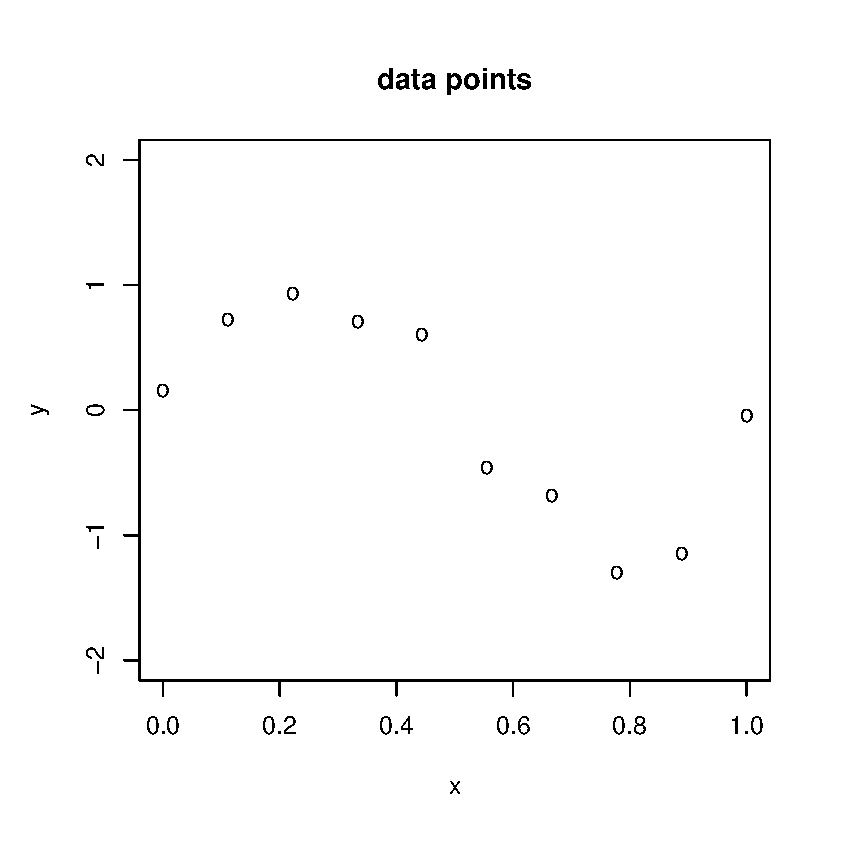
\includegraphics[width=2.0in]
{02Background/bgCurveFit01.eps}
\end{center}
\caption{จุดข้อมูลตัวอย่าง $10$ จุด}
\label{fig: curve fitting 10 datapoints}
\end{figure}
%

ตัวอย่างง่ายๆของการประมาณค่าของฟังชั่นไซ $\xi(x)$ โดยที่ไม่รู้กระบวนการภายในของฟังชั่นไซ 
แต่มีตัวอย่างค่าอินพุต ได้แก่ $x_1, x_2, \ldots, x_N$ 
และตัวอย่างเอาท์พุตจากฟังชั่นไซ ได้แก่ $t_1, t_2, \ldots, t_N$.
นั่นคือ เรารู้ว่า $t_1$ ได้จาก $\xi(x_1)$, 
$t_2$ ได้จาก $\xi(x_2)$, 
$t_3$ ได้จาก $\xi(x_3)$,
$\ldots$,
$t_N$ ได้จาก $\xi(x_N)$.
%
ถึงแม้เราจะไม่รู้สมการ หรือโครงสร้าง หรือกระบวนการภายในฟังชั่นไซจริงๆ 
แต่เราสามารถประมาณฟังชั่นไซได้ด้วยการจำลองพฤติกรรมของฟังชั่นไซจากข้อมูลที่มีเหล่านี้.

%และ เราต้องการประมาณค่าของฟังชั่นไซนี้.
รูปที่~\ref{fig: curve fitting 10 datapoints} แสดงตัวอย่างข้อมูล $10$ จุดข้อมูล ได้แก่ $(x_1, t_1), (x_2, t_2), \ldots, (x_{10}, t_{10})$.
ตัวอย่างนี้ ฟังชั่นไซถูกสร้างมาจาก 
%
\begin{eqnarray}
\xi(x) = \sin(2 \pi x) + \epsilon
\label{eq: bg sin generation}
\end{eqnarray}
%
โดย $\epsilon$ เป็นค่าสุ่มที่มีการกระจายแบบเกาส์ที่ค่าเฉลี่ยเป็น $0$ และ ค่าเบี่ยงเบนมาตราฐานเป็น $0.3$, เขียนย่อๆคือ $\epsilon \sim
\mathcal{N}(\mu=0, \sigma=0.3)$.
เส้นทึบในรูป~\ref{fig: curve fitting 10 datapoints with generating process} แสดงกระบวนการภายในของฟังชั่นที่ต้องการเลียนแบบ.

{\small
\begin{shaded}
ในทางปฏิบัติ เราจะไม่รู้กระบวนการภายในของฟังชั่นที่ต้องการเลียนแบบนี้ เพราะหากเรารู้กระบวนการภายในนี้
เราก็สามารถสร้างโมเดลหรือการจำลองสมการจากกระบวนการภายในที่รู้นี้ได้เลย.
การศึกษาถึงลักษณะปกติ หรือโครงสร้าง หรือกระบวนการภายในจริงๆนี้ 
ต้องอาศัยความเข้าใจเหตุและผล ปฏิสัมพันธ์ พฤติกรรม ปัจจัยที่เกี่ยวข้อง และอาจต้องการการทดลอง ทดสอบ วิเคราะห์ ทบทวนปรับปรุง ซึ่งเป็นกระบวนการทางวิชาการ และหลักการศึกษาวิจัยเฉพาะสำหรับงานแต่ละด้าน แต่ละแขนง แต่ละศาสตร์ ซึ่งต้องอาศัยผู้เชี่ยวชาญเฉพาะด้าน และมักใช้ทรัพยากรและเวลาในการทำมาก.
เทคนิคที่อภิปราย ณ ที่นี้แสดงวิธีที่ใช้การประมาณฟังชั่นที่สนใจ โดยอาศัยเพียงข้อมูลตัวอย่าง ซึ่งเป็นแนวทางหนึ่งที่ให้ผลดีมากในทางปฏิบัติ.
\underline{หมายเหตุ} เทคนิคการประมาณฟังชั่นแบบนี้ ไม่ได้เป็นแนวทางที่จะแข่งขัน 
หรือแทนที่การศึกษาเพื่อเข้าใจถึงโครงสร้างหรือกระบวนการภายใน 
ซึ่งเป็นหัวใจของศาสตร์ต่างๆ แต่เป็นเสมือนเครืองมือที่เสริมเพิ่มเติมขึ้นมา.
นอกจากนั้น ทั้งการประมาณฟังชั่นและการศึกษาถึงความเข้าใจอย่างถ่องแท้ถึงโครงสร้างกระบวนการภายใน 
ยังอาจช่วยซึ่งกันและกัน ช่วยให้ทั้งงานการประมาณฟังชั่นทำได้มีประสิทธิภาพมากขึ้น 
และงานการศึกษาโครงสร้างกระบวนการภายในทำได้สะดวกรวดเร็วมากยิ่งขึ้น.
\end{shaded}
}%small

ตัวอย่างนี้มีลักษณะหลายอย่างที่คล้ายกับชุดข้อมูลจริงๆ 
คือ จุดข้อมูลจะช่วยบอกลักษณะปกติ (Regularity) ของกระบวนเบื้องหลัง (เส้นสีแดง) 
ในขณะเดียวกัน แต่ละจุดข้อมูลจะมีสัญญาณรบกวน (Noise) ปนอยู่.
สัญญาณรบกวนนี้ ($\epsilon$ ในสมการ~\ref{eq: bg sin generation}) อาจจะมาจากธรรมชาติของกระบวนการที่สังเกตุ 
ซึ่งสัญญาณรบกวนอาจมีลักษณะเชิงสุ่ม เช่น การเสื่อมสลายของกัมมันตรังสี, 
หรืออาจจะมาจากความหลากหลายของลักษณะบางอย่างที่ไม่ได้วัด เช่น ความยาวของเมล็ดข้าวของสายพันธ์ุเดียวกัน อาจแปรผันหลายค่า ที่อาจจะมาจากปริมาณน้ำ สารอาหาร แสงแดด ที่ต้นข้าวได้รับ ซึ่งเป็นข้อมูลที่ไม่ได้วัด, 
หรืออาจจะมาจากธรรมชาติของกระบวนการวัดและสังเกตุเองก็เป็นได้.

เป้าหมายของตัวอย่างนี้ก็คือ สามารถทำนาย\textit{ค่าประมาณเอาท์พุต} $\hat{t}$ ของอินพุต $\hat{x}$ ได้ 
แม้อินพุต $\hat{x}$ จะเป็นค่าใหม่ที่ไม่เคยเห็นมาก่อน.
ซึ่งจะว่าไปแล้ว มันก็คือ การหาลักษณะปกติ $\sin(2 \pi x)$ เส้นทึบสีแดงในรูป~\ref{fig: curve fitting 10 datapoints with generating process} นั่นเอง.
%
สำหรับเรื่องการทำนายค่าเอาท์พุตของอินพุตค่าใหม่ที่ไม่เคยเห็นมาก่อน 
เมื่อกล่าวถึง\textit{อินพุตค่าใหม่ที่ไม่เคยเห็นมาก่อน} 
ทั่วๆไปนั้นหมายถึงอินพุตอะไรก็ได้ที่ไม่ซ้ำกับตัวอย่าง.
%
ตัวอย่างของจุดข้อมูล $10$ จุดที่แสดงในรูป~\ref{fig: curve fitting 10 datapoints} 
มีค่าอินพุตและเอาต์พุตดังนี้
\begin{verbatim}
> x
 [1] 0.0000000 0.1111111 0.2222222 0.3333333 0.4444444
 [6] 0.5555556 0.6666667 0.7777778 0.8888889 1.0000000
> t
 [1]  0.16004540  0.72357142  0.93128763  0.71170076
 [5]  0.60979515 -0.46044723 -0.68360173 -1.29926264
 [9] -1.14706643 -0.04490931
\end{verbatim}
%แม้เราจะไม่รู้%
%\footnote{สมมติว่าเราไม่รู้.
%การทำงานกับชุดข้อมูลจริง เราจะไม่รู้กระบวนการเบื้องหลังที่ให้ข้อมูลออกมา.
%}%
%กระบวนการเบื้องหลัง $\xi(x)$ ที่สร้างข้อมูลชุดนี้ขึ้นมา แต่เราสามารถใช้จุดข้อมูล 10 จุดนี้สร้างโมเดลเพื่อทำนายค่าเอาท์พุต ของ
อินพุตใหม่ๆที่ไม่เคยเห็นมาก่อน เช่น $x = 0.1$, $x = 0.5$, $x = 0.9$, เป็นต้น.
แต่ $x = 0$, $x = 0.1111111$, $x = 0.2222222$, ..., $x = 1$  ไม่ใช่อินพุตใหม่ๆ 
เพราะค่าเหล่านี้มีอยู่ในตัวอย่างแล้ว.

%
\begin{figure}
\begin{center}
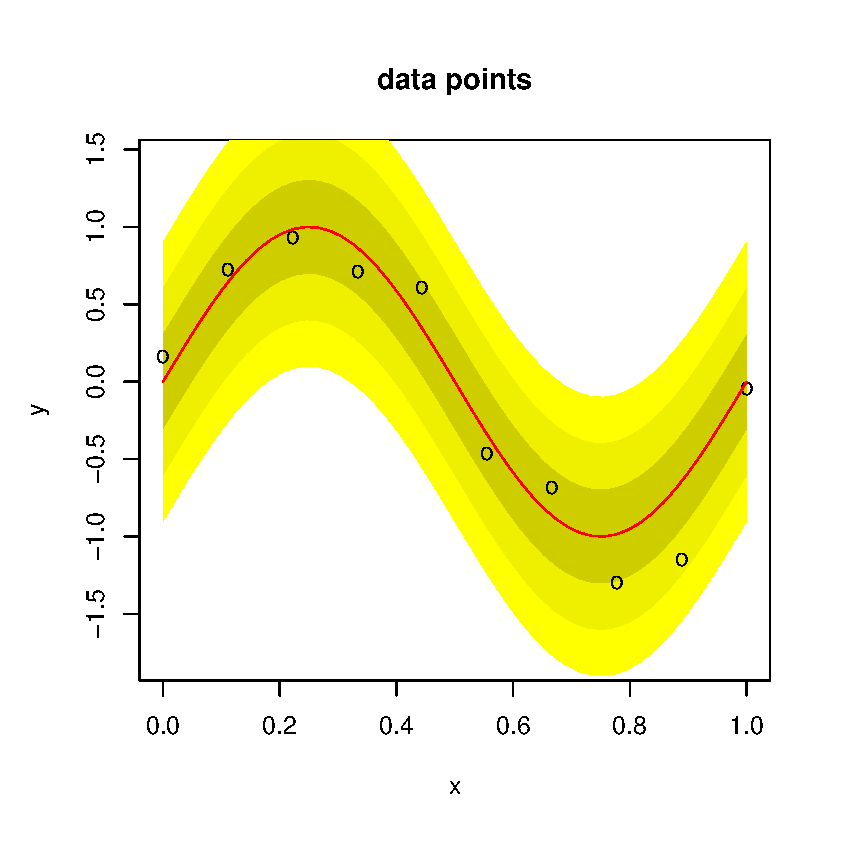
\includegraphics[width=2.0in]
{02Background/bgCurveFit02.eps}
\end{center}
\caption{จุดข้อมูลตัวอย่าง $10$ จุด พร้อม เส้นทึบสีแดงแสดงค่าลักษณะปกติ $\sin(2 \pi x)$ (โครงสร้างภายในที่สร้างข้อมูลออกมา โดยปราศจากสัญญาณรบกวน) 
และพื้นที่สีเหลืองแสดงบริเวณที่ห่างจากค่าลักษณะปกติ $\sin(2 \pi x)$ เป็นระยะ $\sigma$, $2 \sigma$, และ $3 \sigma$ ตามลำดับความเข้มของสี}
\label{fig: curve fitting 10 datapoints with generating process}
\end{figure}
%

\paragraph{โมเดลฟังชั่นพหุนาม.}
ตัวอย่างนี้แสดงการประมาณค่าเอาท์พุต โดยการสร้างโมเดลขึ้นมา
ซึ่งสำหรับบทนี้จะใช้ \textit{ฟังชั่นพหุนาม} (Polynomial Function) เป็นโมเดล.\index{Polynomial Function}
%
ฟังชั่นพหุนามอธิบายความสัมพันธ์ระหว่างเอาต์พุตกับอินพุต ดังนี้
\begin{eqnarray}
   y(x, \mathbf{w}) = w_0 + w_1 \cdot x + w_2 \cdot x^2 + \cdot + w_M \cdot x^M = \sum_{j=0}^M w_j x^j
\label{eq: bg polynomial}
\end{eqnarray}
โดย ค่าของฟังชั่น $y$ คือค่าประมาณเอาท์พุต,
ตัวแปร $x$ แทนค่าอินพุตที่สงสัย,
ตัวแปร $M$ เป็น\textit{ลำดับ} (order) ของฟังชั่นพหุนาม 
และ ตัวแปร $w_0, w_1, w_2, \ldots, w_M$ คือค่าสัมประสิทธิ์ต่างๆของพหุนาม 
และกรณีนี้ ก็เป็น\textit{พารามิเตอร์ของโมเดล}ด้วย.
เพื่อความสะดวก บางครั้งเราจะอ้างถึงด้วยพารามิเตอร์ $w_0, w_1, w_2, \ldots, w_M$ หลายๆตัวนี้ ด้วยตัวแปร $\mathbf{w}$.

รูปกราฟของฟังชั่นพหุนามสามารถปรับเปลี่ยนรูปทรงได้ตามความซับซ้อนของฟังชั่น (ระบุโดย\textit{ลำดับพหุนาม} $M$) และ\textit{ค่าของพารามิเตอร์} $\mathbf{w}$.
รูป~\ref{fig: various shapes of polynomial} แสดงตัวอย่างรูปทรงของกราฟจากฟังชั่นพหุนามที่ลำดับและพารามิเตอร์ค่าต่างๆ.
สังเกตุว่ายิ่งค่า\textit{ลำดับพหุนาม}ยิ่งมาก ฟังชั่นพหุนามก็จะมี\textit{ระดับของอิสรภาพ} (Degree of Freedom) มากตามไปด้วย.
นั่นคือ หาก $M = 0$ ฟังชั่นพหุนามสามารถแสดงเป็นเส้นตรงแนวนอนได้เท่านั้น,
หาก $M = 1$ ฟังชั่นพหุนามสามารถแสดงเป็นเส้นตรงที่ความชันต่างๆได้ด้วย,
หาก $M = 2$ ฟังชั่นพหุนามเพิ่มความสามารถที่จะโค้งงอได้ $1$ งอ,
หาก $M = 3$ ฟังชั่นพหุนามเพิ่มความสามารถที่จะโค้งงอได้ $2$ งอ
เช่นนี้ เป็นต้น
%
\begin{figure}
\begin{center}
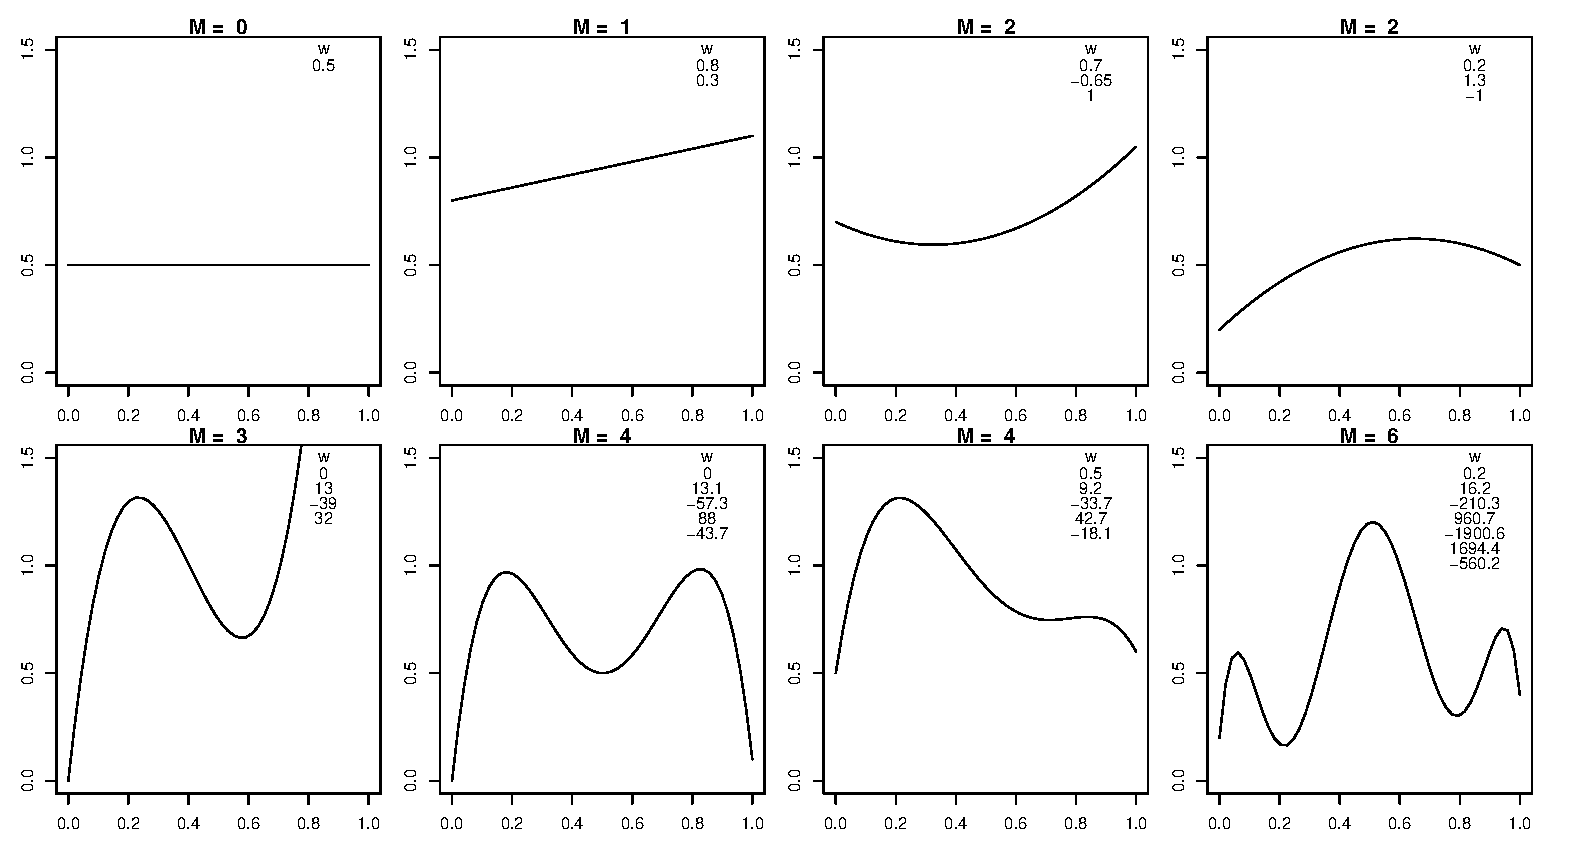
\includegraphics[width=5.5in]
{02Background/bgPolynomial.eps}
\end{center}
\caption{รูปทรงต่างๆของฟังชั่นพหุนามปรับเปลี่ยนไปตาม\textit{ลำดับของพหุนาม}
และ\textit{ค่าของพารามิเตอร์}.}
\label{fig: various shapes of polynomial}
\end{figure}
%

\paragraph{การฝึกโมเดล.}
\index{training}
\index{learning}
\index{การฝึกโมเดล}

การฝึกโมเดล (Training) หรือการให้โมเดลเรียน (Learning) ก็คือการปรับค่าพารามิเตอร์ $\mathbf{w}$ เพื่อให้โมเดลสามารถประมาณฟังชั่นที่สนใจได้
โดยจะใช้\textit{ตัวอย่างที่มี}มาช่วยปรับค่าพารามิเตอร์ เพื่อให้เอาท์พุตของโมเดลใกล้กับเอาท์พุตของตัวอย่างมากที่สุด สำหรับที่ค่าอินพุตเดียวกัน.

การวัดความใกล้ระหว่าง\textit{เอาท์พุตของโมเดล}กับ\textit{เอาท์พุตของตัวอย่าง}
จะใช้ค่าผลต่างกำลังสอง (สมการ~\ref{eq: bg curve fitting E})

\begin{eqnarray}
E(\mathbf{w}) = \frac{1}{2} \sum_{n=1}^N \{ y(x_n, \mathbf{w}) - t_n \}^2
\label{eq: bg curve fitting E}
\end{eqnarray}
โดย ตัวเลข $\frac{1}{2}$ นี้ใส่เพื่อความสะดวก ซึ่งจะได้เห็นต่อไปในขั้นตอนการหาอนุพันธ์.
%
ฟังชั่นเป้าหมาย (สมการ~\ref{eq: bg curve fitting E}) นี้อาจจะเรียกว่า \textit{ฟังชั่นค่าผิดพลาด} (Error Function) หรือ\textit{ฟังชั่นค่าใช้จ่าย} (Cost Function).
\index{Error Function}
\index{Cost Function}
%
ถ้าค่าที่ทำนายผิดจากค่า\textit{เอาท์พุตของตัวอย่าง}มาก ค่าผลต่างกำลังสองก็จะมากตามไปด้วย.
หรือ ถ้าค่าที่ทำนายผิดจากเป้าหมายน้อย ค่าผลต่างกำลังสองก็จะน้อย.
รูปที่~\ref{fig: bg MSE} แสดงค่าผลต่างกำลังสอง สำหรับผลของการทำนายแบบต่างๆ.

%
\begin{figure}
\begin{center}
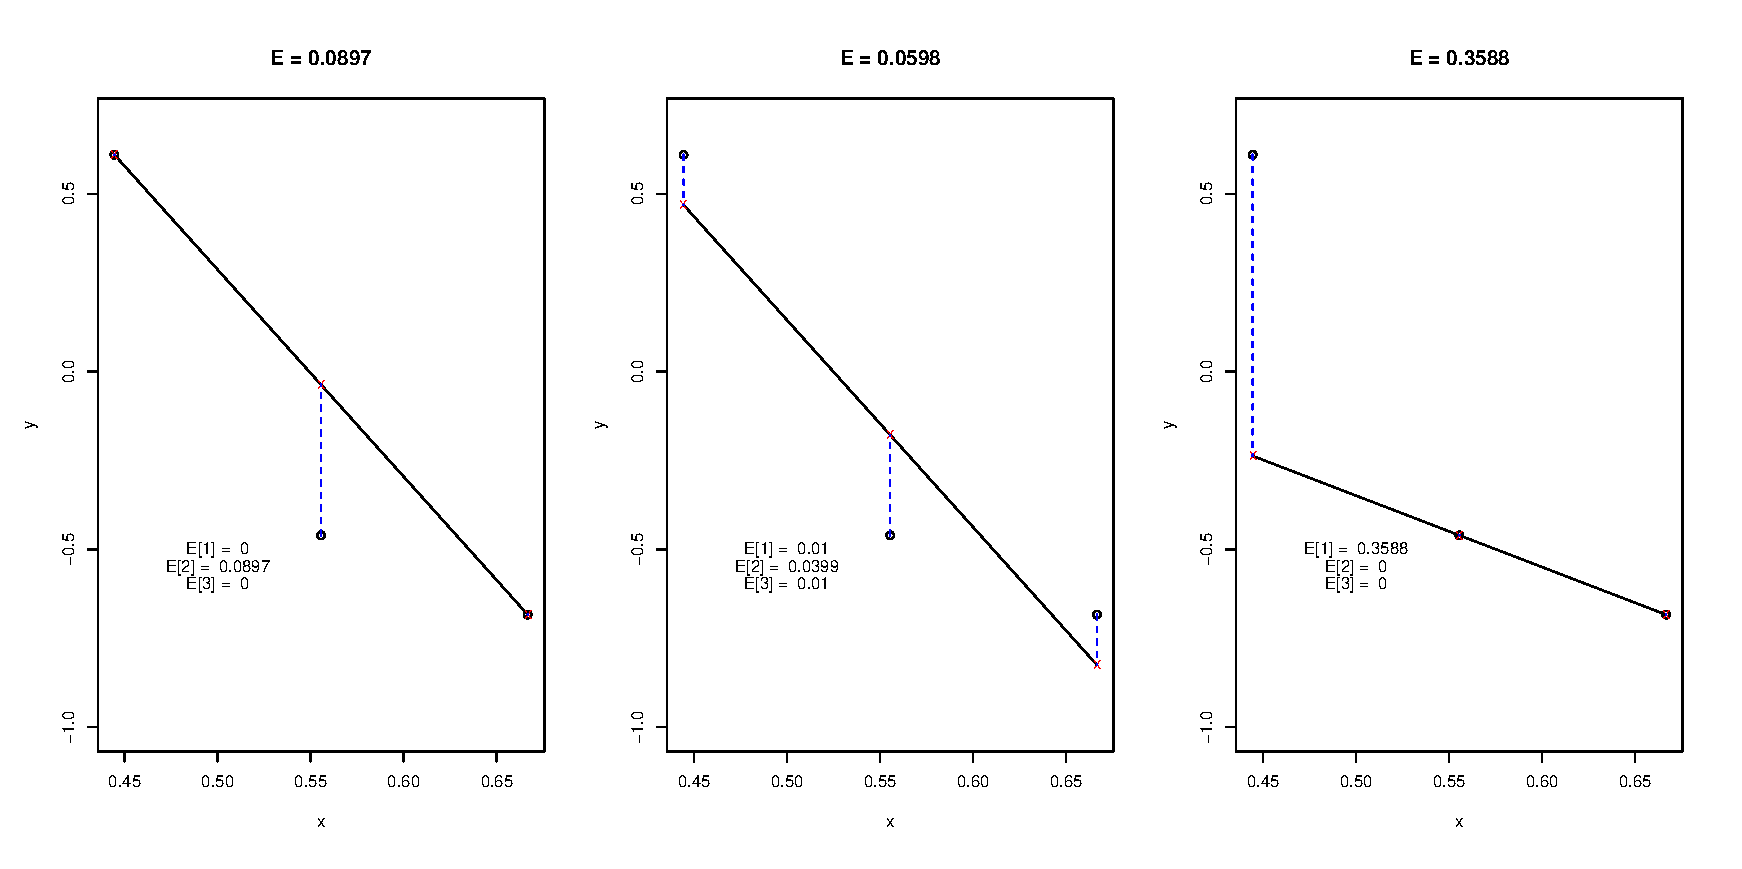
\includegraphics[width=5.5in]{02Background/bgMSE.eps}
\end{center}
\caption{ค่าผลต่างกำลังสองสำหรับผลทำนายจากโมเดลแบบต่างๆ ซึ่งทำนายค่าจุดตัวอย่าง $3$ จุด.
จุดข้อมูลตัวอย่างแสดงด้วยวงกลม.
กากบาทแทนค่าเอาต์พุตจากโมเดล (ค่าทำนาย).
เส้นทึบแสดงให้เห็นค่าฟังชั่นของโมเดลตลอดช่วงค่าที่แสดง.
เส้นประแสดงระยะห่างระหว่าง\textit{ค่าทำนายที่เป็นเอาต์พุตจากโมเดล}และ\textit{ค่าตัวอย่างจากจุดข้อมูล}ที่อินพุตเดียวกัน.
ภาพซ้าย โมเดลทายจุดข้อมูลที่ 1 และ 3 ได้อย่างแม่นยำ \texttt{E[1]=0} และ \texttt{E[3]=0}
แต่ทายจุดข้อมูลที่ 2 ผิดไป โดยทายค่ามากเกินไป ซึ่งผลรวมของระยะห่างทั้งสามจะได้ \texttt{E = 0.0897}.
ภาพกลาง โมเดลทายจุดข้อมูลทั้ง $3$ ผิดไปบ้าง โดยทายค่าจุดที่ 1 และ 3 ต่ำเกินไป แต่ทายจุดที่ 2 สูงเกินไป
และได้ผลรวมของระยะห่างทั้งสาม \texttt{E = 0.0598}.
ภาพขวา โมเดลทายจุดข้อมูล 1 ผิดไปมาก แต่ทายจุดที่ 2 และ 3 ได้อย่างแม่นยำ
และได้ผลรวมของระยะห่างทั้งสาม \texttt{E = 0.3588}.
การใช้\textit{ผลรวมของระยะห่าง}ในการวัดคุณภาพของโมเดล เช่นนี้เพื่อให้สามารถสะท้อนความสามารถในการทำนายได้ดีสำหรับทุกๆจุดข้อมูล
ซึ่งเชื่อว่าน่าจะช่วยสะท้อนคุณภาพการเลียนแบบกระบวนการเบื้องหลังที่สนใจได้ดี}
\label{fig: bg MSE}
\end{figure}
%

การทำนายค่าเอาท์พุตที่เป็นค่าต่อเนื่องแบบนี้ จะเรียกว่า \textit{การหาค่าถดถอย} (Regression), ซึ่งจะต่างจาก\textit{การจำแนกประเภท} (Classification) ที่ค่าของเอาต์พุตจะจำกัดอยู่เฉพาะค่าในเซตของคำตอบที่กำหนด 
(การจำแนกประเภทจะอภิปรายในหัวข้อ~\ref{section: Logistic Regression}).
ค่าความใกล้ หรือ ค่าฟังชั่นค่าผิดพลาด $E$ นี้ สำหรับ\textit{การหาค่าถดถอย}จะเรียกว่าสั้นๆว่า \textit{ค่าความผิดพลาด} (Error).

ทบทวนคำนิยามของการเรียนรู้ของเครื่องโดย ทอม มิชเชล\cite{Mitchell1997a}, การหาค่าถดถอยนี้ จัดเป็นวิธีการเรียนรู้ของเครื่อง โดย ประสบการณ์คือการสังเกตุอินพุตและเอาท์พุตของตัวอย่าง, 
งานคือการทำนายค่าเอาท์พุต ตามค่าอินพุต, 
และตัววัดผลการทำงานคือค่าความผิดพลาดของการทำนาย ตามสมการ~\ref{eq: bg curve fitting E}.

\subsection{ฝึกโมเดลฟังชั่นพหุนามอันดับหนึ่ง}
ตัวอย่างนี้เลือกฟังชั่นพหุนามอันดับ 1. 
นั่นคือ $y(x, \mathbf{w}) = w_0 + w_1 x$ ในการทำนายค่าฟังชั่นไซ
โดยจะเลือกค่า $w_0$ และ $w_1$ จากค่าที่ให้ความผิดพลาดต่ำสุดของการทำนายข้อมูลตัวอย่าง $N=10$ จุดข้อมูล.
ค่าความผิดพลาดต่ำสุดที่เป็นไปได้จะเกิดขึ้นเมื่อ $\frac{\partial E}{\partial w_0} = 0$ 
และ $\frac{\partial E}{\partial w_1} = 0$.
(ดูหัวข้อ~\ref{section: Optimization} สำหรับทบทวนการหาค่าดีที่สุด)
เมื่อแทนค่า $E$ จากสมการ~\ref{eq: bg curve fitting E} จะได้

\begin{eqnarray}
%\frac{\partial E}{\partial w_0} &=& 0
%\label{eq: bg polynomial derivatives 1a} \\
%\frac{\partial E}{\partial w_1} &=& 0
%\label{eq: bg polynomial derivatives 1b} \\
\frac{\partial \frac{1}{2} \sum_{n=1}^N \{ w_0 + w_1 x_n - t_n \}^2}{\partial w_0} &=& 0, 
\label{eq: bg polynomial derivatives 2a}
\\
\frac{\partial \frac{1}{2} \sum_{n=1}^N \{ w_0 + w_1 x_n - t_n \}^2}{\partial w_1} &=& 0
\label{eq: bg polynomial derivatives 2b}
\end{eqnarray}

และเมื่อทำอนุพันธ์เสร็จจะได้
\begin{eqnarray}
\sum_{n=1}^N \{ (w_0 + w_1 x_n - t_n) \cdot (1 + 0 - 0) \} &=& 0, 
\label{eq: bg polynomial derivatives 3a} \\
\sum_{n=1}^N \{ (w_0 + w_1 x_n - t_n) \cdot (0 + x_n - 0) \} &=& 0.
\label{eq: bg polynomial derivatives 3b}
\end{eqnarray}

หลังจากจัดรูปใหม่ โดยเรียงตามพารามิเตอร์ จะได้
\begin{eqnarray}
%
  w_0 \sum_{n=1}^N \{ 1 \} + w_1 \sum_{n=1}^N \{ x_n \} - \sum_{n=1}^N \{ t_n \} &=& 0, 
\label{eq: bg polynomial derivatives 4a} \\
  w_0 \sum_{n=1}^N \{ x_n \} + w_1 \sum_{n=1}^N \{ x_n^2 \} - \sum_{n=1}^N \{ t_n \cdot x_n \} &=& 0 
\label{eq: bg polynomial derivatives 4b}
\end{eqnarray}
ซึ่งเมื่อจัดรูปสมการ~\ref{eq: bg polynomial derivatives 4a} และ~\ref{eq: bg polynomial derivatives 4a} ให้อยู่ในรูปเมตริกซ์จะได้
\begin{eqnarray}
%
\left[ 
\begin{matrix}
N & \sum_{n=1}^N x_n \\
\sum_{n=1}^N x_n & \sum_{n=1}^N x_n^2
\end{matrix}
\right] \cdot 
\left[ 
\begin{matrix}
w_0 \\
w_1
\end{matrix}
\right]
=
\left[ 
\begin{matrix}
\sum_{n=1}^N t_n \\
\sum_{n=1}^N t_n \cdot x_n
\end{matrix}
\right].
\label{eq: bg polynomial M1}
\end{eqnarray}

จากค่าจุดข้อมูลในหัวข้อ~\ref{section: Polynomial Curve Fitting}, นั่นจะได้ $N = 10$, $\sum_{n=1}^N x_n = 5$, $\sum_{n=1}^N x_n^2 = 3.519$, $\sum_{n=1}^N t_n = -0.499$, และ $\sum_{n=1}^N t_n x_n = -1.991$.
เมื่อแก้สมการแล้วจะได้ค่า 
\[
[w_0, \; w_1]^T = [0.805, \; -1.709]^T.
\]

แนวทางที่ทำนี้เรียกว่า \textit{วิธีกำลังสองน้อยที่สุด} (Least Squares Method) ซึ่งคือ 
การหาค่าของพารามิเตอร์ที่ทำให้ค่าทำนายผิดพลาดกำลังสองมีค่าน้อยที่สุด
หรือ การหาค่าของพารามิเตอร์ที่เป็นตัวทำน้อยที่สุดของฟังชั่นค่าผิดพลาด.
นั่นคือ การหา 
\[
\mathbf{w}^\ast = \arg\min_{\mathbf{w}} \frac{1}{2} \sum_n \{y(\mathbf{x}_n, \mathbf{w}) - t_n\}^2.
\]

\subsection{การใช้โมเดลฟังชั่นพหุนาม}
หลังจากได้ค่าพารามิเตอร์ที่เหมาะสมมาแล้ว (เช่น $[w_0, \; w_1]^T = [0.805, \; -1.709]^T$) ค่าประมาณของฟังชั่นก็สามารถคำนวณได้จากโมเดลที่แทนค่าพารามิเตอร์เหล่านั้น $y = 0.805 + -1.709 x$.
รูป~\ref{fig: bg curve fitting M1} แสดงจุดข้อมูลและผลทำนายจากโมเดลหลังจากกระบวนการฝึกโมเดล.

%
\begin{figure}
\begin{center}
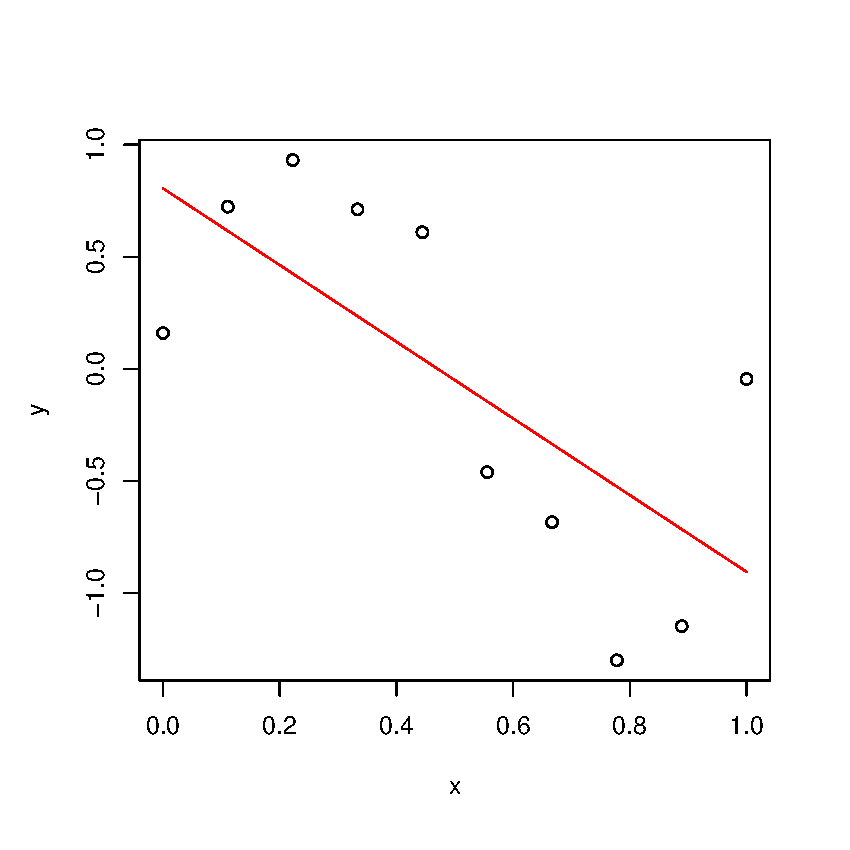
\includegraphics[height=3.0in]{02Background/bgCurveFittingM1.eps}
\end{center}
\caption{ผลจากโมเดลพหุนามอันดับหนึ่งที่ฝึกแล้ว (เส้นสีแดง)}
\label{fig: bg curve fitting M1}
\end{figure}
%

\subsection{กิจกรรมปฏิบัติลองโปรแกรมหาค่าถดถอยด้วยฟังชั่นพหุนาม}

\begin{verse}
``ไม่ว่าบทกวีจะบรรยายกลิ่นรสชาติของมะม่วงว่า อร่อย หอม หวาน เพียงใด\\
ผู้อ่านก็ไม่อาจเข้าใจได้ดีเท่ากับได้ลิ้มลองชิมรสด้วยตนเอง\\
เช่นเดียวกัน 
การอ่านหรือฟังทฤษฎีการเรียนรู้ของเครื่องมากเท่าใด
ก็ไม่อาจช่วยให้เข้าใจได้เท่ากับลองประสบการณ์ด้วยตนเอง'' \\
---ผู้เขียน
\end{verse}


หัวข้อนี้ให้ตัวอย่าง เพื่อผู้อ่านสามารถนำไปทดลองลงมือปฎิบัติ 
เพื่อช่วยให้เข้าใจการทำงานของการสร้างโมเดลฟังชั่นพหุนาม
และการใช้โมเดลในการทำนาย
ซึ่งเป็นพื้นฐานเบื้องต้นสำหรับศาสตร์การเรียนรู้ของเครื่อง.

โค้ดข้างล้างนี้ใช้เพื่อสร้างจุดข้อมูล $10$ จุด โดยแต่ละจุดข้อมูลมีค่าอินพุตตั้งแต่ $0$ ถึง $1$ 
และความสัมพันธ์ระหว่างอินพุตกับเอาต์พุตคือ $y = \sin(2 \pi x) + \epsilon$ 
โดย $\epsilon$ แทนสัญญาณรบกวน (ในโค้ดทำสัญญาณรบกวนด้วย \texttt{rnorm})
\begin{verbatim}
N = 10;
dp.x <- seq(0, 1, len=N)
dp.t <- sin(2*pi*dp.x) + rnorm(10, mean=0, sd=0.3)
\end{verbatim}

โค้ดข้างล่างนิยามฟังชั่น \texttt{w.polyfit1}  
สำหรับ\textit{ฝึกโมเดล}(หาค่าพารามิเตอร์).
สังเกตุเมตริกซ์ \texttt{A} และเวคเตอร์ \texttt{b} เปรียบเทียบกับสมการ~\ref{eq: bg polynomial M1}.

\begin{verbatim}
w.polyfit1 <- function(xn, tn){
# xn and tn are training data.
	
   N <- length(xn)

   sumx <- sum(xn)
   sumx2 <- sum(xn^2)
   sumt <- sum(tn)
   sumtx <- sum(tn*xn)

   A <- matrix(c(N, sumx, sumx, sumx2), 2, 2, byrow=T )
   b <- matrix(c(sumt, sumtx), 2, 1)
   
   w <- solve(A,b)
   
return(w)
}##end w.polyfit1
\end{verbatim}

โค้ดข้างล่างนิยามฟังชั่น \texttt{y.poly1} สำหรับ\textit{ทำนายค่าเอาท์พุต}.
สังเกตุ \texttt{y[i] = w[2]*x[i] + w[1]} ทำการคำนวณโมเดลพหุนามที่ค่า \texttt{x[i]}.

\begin{verbatim}
y.poly1 <- function(x,w){
## w must have length 2: [w0 w1] = c(w[1], w[2])

	N.x <- length(x)
	y <- rep(0, len=N.x)
	for(i in 1:N.x){
	   y[i] = w[2]*x[i] + w[1];
	}##end i
	
return(y)
}## end y.poly1
\end{verbatim}

ข้อมูลตัวอย่างที่สร้างขึ้นมา (อินพุต \texttt{dp.x} และเอาท์พุต \texttt{dp.t}) 
นำมาใช้ฝึกโมเดลเพื่อหาค่าพารามิเตอร์ \texttt{w} ได้ดังนี้

\begin{verbatim}
> w <- w.polyfit1(dp.x, dp.t)
> w
           [,1]
[1,]  0.8050556
[2,] -1.7098887
\end{verbatim}

หลังจากฝึกโมเดลตามขั้นตอนข้างต้นแล้ว 
โมเดลนี้ (สมบูรณ์แล้ว ด้วยค่าพารามิเตอร์ \texttt{w})
สามารถนำไปประมาณค่าเอาท์พุตต่างๆ ที่อินพุต $0.1, 0.25, 0.5, 0.75, 0.9$ 
ดังแสดงในตัวอย่างข้างล่างนี้

\begin{verbatim}
> y.poly1(0.1, w)
[1] 0.6340668
> y.poly1(0.25, w)
[1] 0.3775835
> apply(matrix(c(0.1, 0.25, 0.5, 0.75, 0.9)), 1, y.poly1, w)
[1]  0.6340668  0.3775835 -0.0498887 -0.4773609 -0.7338442
\end{verbatim}
สังเกตุการใช้คำสั่ง \texttt{apply} แทนการเรียกฟังชั่นทีละครั้ง.
ผู้อ่านสามารถเปลี่ยนกระบวนการที่ใช้สร้างจุดข้อมูล และ/หรือ เปลี่ยนค่าจำนวนข้อมูล \texttt{N} 
แล้วทดลองฝึกโมเดลและใช้โมเดลที่ฝึกประมาณค่าเอาท์พุตที่สร้างใหม่ เพื่อความเข้าใจที่ดีขึ้นได้.

\section{การเลือกโมเดล}
\label{section: Model selection}
%\footnote{แนะนำให้ทำแบบฝึกหัดท้ายบทข้อ 1 ถึง 9 ก่อน}

สำหรับข้อมูลชุดหนึ่ง เราสามารถใช้โมเดลต่างๆกันเพื่อประมาณข้อมูลชุดนั้นได้  เช่น เราสามารถใช้โมเดลฟังชั่นพหุนามอันดับต่างๆ เพื่อประมาณจุดข้อมูล ดังแสดงในรูป~\ref{fig: bg poly curve fitting Ms}.
สังเกตุพหุนามอันดับ 9 ผ่านจุดข้อมูลทุกจุด แต่รูปทรงกราฟจากโมเดลจะเปลี่ยนแปลงเร็วมาก.
โดยทั่วไปแล้ว พหุนามอันดับ 9 สามารถผ่านจุดข้อมูล $10$ จุดที่ใช้ฝึกได้ทุกจุด.
\underline{หมายเหตุ} พหุนามอันดับ 9 มี\textit{ดีกรีของความเป็นอิสระเป็น} $10$ ($10$ Degrees of Freedom, การที่สามารถควบคุมด้วยสัมประสิทธิ์ $10$ ค่า $w_0, \ldots, w_9$ ได้). 

แต่หากได้ข้อมูลมาเพิ่ม (หรืออาจจะเป็นจุดข้อมูลที่กันไว้แต่แรก) ดังรูป~\ref{fig: bg train and test datapoints}
แล้วเมื่อประเมินค่าความผิดพลาดจากการทำนายด้วยโมเดลพหุนามที่ดีกรีต่างๆ
จะได้ผลดังแสดงในรูป~\ref{fig: bg train and test RMSEs}.

%
\begin{figure}
\begin{center}
\includegraphics[height=3.0in]{02Background/bgPolyMs.eps}
\end{center}
\caption{ผลจากโมเดลพหุนามอันดับต่างๆกัน (เส้นทึบสีแดง) 
และค่าของฟังชั่นที่ใช้สร้างจุดข้อมูลเมื่อไม่มีสัญญาณรบกวน (เส้นประสีน้ำเงิน)}
\label{fig: bg poly curve fitting Ms}
\end{figure}
%

%
\begin{figure}
\begin{center}
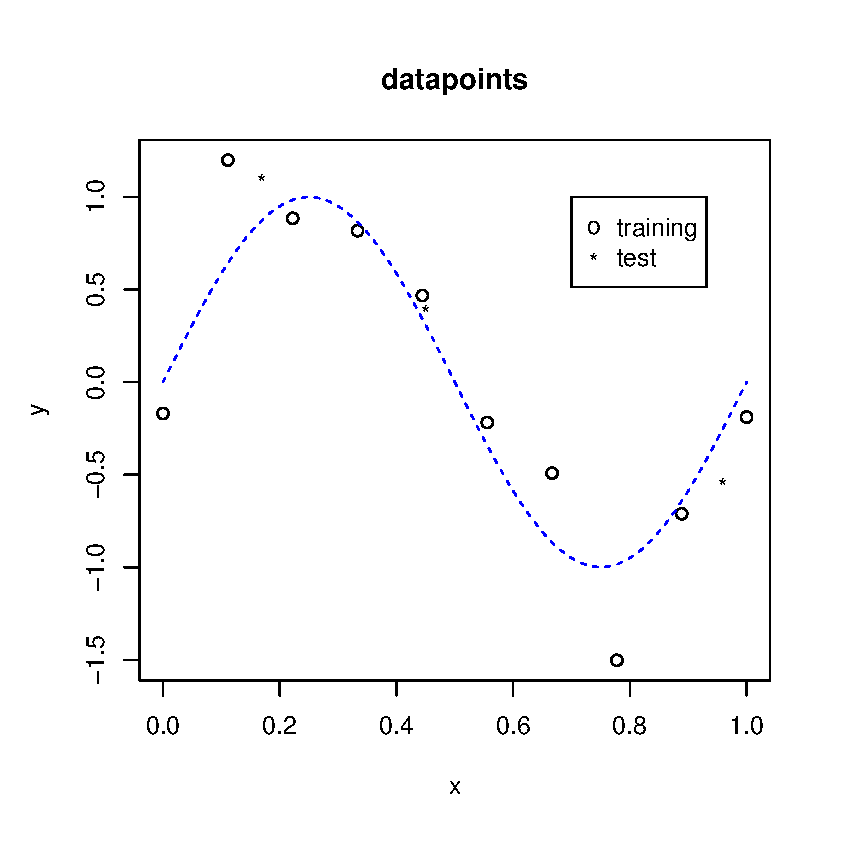
\includegraphics[height=3.0in]{02Background/bgAddTestPoints.eps}
\end{center}
\caption{จุดข้อมูลที่ใช้ฝึกโมเดลและจุดที่ใช้ทดสอบ}
\label{fig: bg train and test datapoints}
\end{figure}
%

%
\begin{figure}
\begin{center}
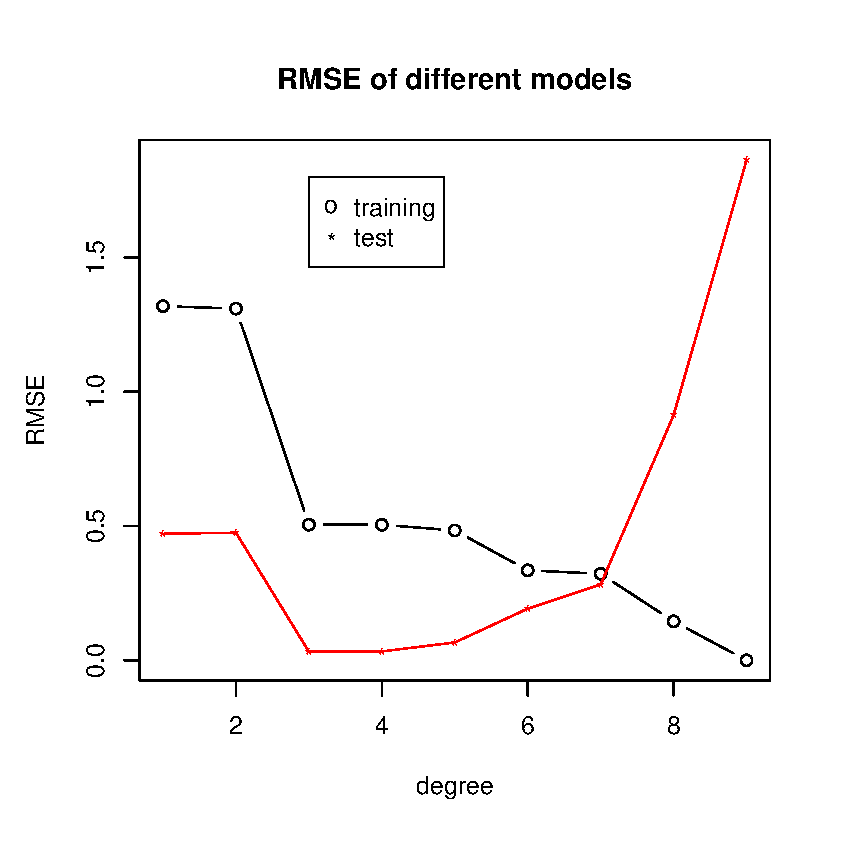
\includegraphics[height=3.0in]{02Background/bgModelEval.eps}
\end{center}
\caption{ผลจากค่าผิดพลาดแบบ\textit{อาร์เอมเอส}ของโมเดลพหุนามที่ดีกรีต่างๆ
กับชุดข้อมูลที่ใช้ฝึก (แทนด้วยสัญญลักษณ์ `o')
กับชุดข้อมูลทดสอบ (แทนด้วยสัญญลักษณ์ `*')}
\label{fig: bg train and test RMSEs}
\end{figure}
%

จากค่าความผิดพลาดจากการทำนายด้วยโมเดลพหุนามในรูป~\ref{fig: bg train and test RMSEs} แสดงให้เห็นว่า การทำนายข้อมูลชุดฝึก (สัญญลักษณ์ `o') ค่าความผิดพลาดลดลงเรื่อยๆ เมื่อดีกรีของพหุนามเพิ่มขึ้น (เทียบเท่ากับการใช้โมเดลที่มีความซับซ้อนสูงขึ้น).
แต่การทำนายข้อมูลชุดทดสอบ (สัญญลักษณ์ `*') ลดลงช่วงแรก แล้วเพิ่มขึ้นอย่างมากในช่วงหลัง.

จริงๆแล้ว พหุนามดีกรีที่สูงกว่า สามารถที่จะทำตัวเสมือนเป็น ดีกรีที่ต่ำกว่าได้ โดยการปรับให้ค่าสัมประสิทธิที่เทอมกำลังสูงๆเป็นศูนย์.
กล่าวอย่างง่ายคือ พหุนามดีกรีที่สูงกว่าสามารถที่จะให้ผลการทำนายที่ไม่แย่ไปกว่าพหุนามที่ดีกรีต่ำกว่าได้.
ยิ่งกว่านั้น สำหรับตัวอย่างนี้ เราอาจบอกได้ว่า โมเดลที่จะทำนายข้อมูลชุดนี้ได้ดีที่สุดคือ โมเดลแทนเส้นประสีน้ำเงิน ในรูป~\ref{fig: bg poly curve fitting Ms} ซึ่ง คือ $\sin(2 \pi x)$  ที่ใช้สร้างจุดข้อมูลขึ้นมา.
และจาก\textit{การขยายของอนุกรมเทย์เลอร์} (Taylor Series Expansion) ของ $\sin(2 \pi x)$ น่าจะให้ผลที่ว่า ผลการทำนายน่าจะยิ่งดีขึ้นเมื่อดีกรีสูงขึ้น (ดูแบบฝึกหัดข้อ 10)
%
เพื่อจะเข้าใจพฤติกรรมการฝึกโมเดล เมื่อพิจารณาค่าของสัมประสิทธิที่ได้จากการฝึกโมเดล ดังแสดงในตาราง~\ref{tbl: bg polynomial coeff}.
จะเห็นว่า เมื่อดีกรีสูงขึ้น ขนาดของค่าสัมประสิทธิก็ใหญ่ขึ้นด้วย.
โดยเฉพาะที่ดีกรี 9 ค่าสัมประสิทธิถูกปรับให้เข้ากับจุดข้อมูลอย่างมาก เห็นได้จากค่าสัมประสิทธิที่มีขนาดใหญ่มากๆ (ค่าลบมากๆ หรือค่าบวกมากๆ) 
ทำให้พหุนามสามารถผ่านจุดข้อมูลได้ทุกจุด
แต่ว่าระหว่างจุดข้อมูล ค่าของพหุนามกลับเปลี่ยนแปลงอย่างรุนแรง (ภาพท้ายสุดของรูป~\ref{fig: bg poly curve fitting Ms}).
สิ่งที่เกิดขึ้นก็คือ โมเดลที่ซับซ้อนสูงได้ปรับตัวให้เข้ากับสัญญาณรบกวนของข้อมูล แทนที่จะปรับให้เข้ากับข้อมูลโดยทั่่วๆไป
ซึ่งแม้จะทำให้โมเดลสามารถทายข้อมูลได้อย่างแม่นยำ แต่ทำให้โมเดลสูญเสียความสามารถในการทำนายข้อมูลอื่นๆ (ที่ไม่ใช้ข้อมูลฝึกหัด)ลดลง.
กรณีที่โมเดลที่ฝึกแล้วปรับตัวไปกับสัญญาณรบกวน จะเรียกว่าเกิด\textit{โอเวอร์ฟิตติ้ง} (Overfitting). \index{overfitting} \index{โอเวอร์ฟิตติ้ง}

\begin{table}[hbtp]
%{\tiny
{\scriptsize
\caption{ค่าสัมประสิทธิของฟังชั่นพหุนามหลังผ่านการฝึก}
\begin{center}
%\begin{tabular}{c|rrrrrrrrrr}
\begin{tabular}{>{\arraybackslash}m{0.1in}|
>{\arraybackslash}m{0.25in}
>{\arraybackslash}m{0.25in} 
>{\arraybackslash}m{0.4in} 
>{\arraybackslash}m{0.4in}
>{\arraybackslash}m{0.42in}
>{\arraybackslash}m{0.42in}
>{\arraybackslash}m{0.42in}
>{\arraybackslash}m{0.42in}
>{\arraybackslash}m{0.42in}
>{\arraybackslash}m{0.42in}
}
%\hline 
$M$ & $w_0$ & $w_1$ & $w_2$ & $w_3$ & $w_4$ & $w_5$ & $w_6$ & $w_7$ & $w_8$ & $w_9$ \\
\hline
1 & 0.83  & -1.64  &  &  &  &  &  &  &  &  \\ 
2 & 0.71  & -0.87  & -0.78  &  &  &  &  &  &  &  \\
3 & -0.06  & 11.89  & -34.39  & 22.41  &  &  &  &  &  &  \\
%-0.07  & 12.17  & -35.82  & 24.71  & -1.15  &  &  &  &  &  & 
%5 & -0.11  & 16.18  & -69.23  & 119.13  & -109.38  & 43.29  &  &  &  &  \\
%6 & -0.17  & 31.54  & -258.76  & 934.91  & -1685.84  & 1445.58  & -467.43  &  &  &  \\
6 & -0.17  & 31.54  & -259  & 935  & -1686  & 1446  & -467  &  &  &  \\
%-0.16  & 24.11  & -136.19  & 208.02  & 369.47  & -1551.66  & 1707.69  & -621.46  &  &  & 
%-0.17  & 78.55  & -1233.92  & 8487.73  & -30865.28  & 63476.09  & -74158.03  & 45826.93  & -11612.1  &  & 
%9 & -0.17  & -18.6  & 1009.96  & -11723.66  & 64085.01  & -195203.42  & 349413.48  & -365010.66  & 205750.66  & -48302.79 \\ %\hline 
9 & -0.17  & -18.6  & 1010  & -11724  & 64085  & -195203  & 349413  & -365011  & 205751  & -48301 \\ %\hline 
\end{tabular} 
\end{center}
\label{tbl: bg polynomial coeff}
}%end \small
\end{table}

รูป~\ref{fig: bg poly M9 different data sizes} แสดงผลการฝึกพหุนามดีกรี 9 ด้วยชุดข้อมูลที่สร้างจากฟังชั่นเดียวกัน แต่ขนาดข้อมูลต่างกัน.
จากรูป~\ref{fig: bg poly M9 different data sizes} จะเห็นว่า ที่พหุนามดีกรีเดิม 
เมื่อจำนวนข้อมูลมากขึ้น ปัญหาโอเวอร์ฟิตติ้งลดลง.
หรือ อาจจะกล่าวอีกอย่างได้ว่า เมื่อมีข้อมูลมากขึ้น เราสามารถใช้โมเดลที่ซับซ้อนมากขึ้นได้.
บิชอบ\cite{Bishop2006a} กล่าวถึงว่า ผู้เชี่ยวชาญบางคนถึงกับแนะนำว่า จำนวนข้อมูลไม่ควรน้อยกว่า $5$ ถึง $10$ เท่าของจำนวนพารามิเตอร์ของโมเดล.

อย่างไรก็ตาม เราไม่ควรจะต้องจำกัดจำนวนพารามิเตอร์ของโมเดลตามขนาดของข้อมูลที่เรามี 
เพราะว่า เราควรจะสามารถเลือกจำนวนพารามิเตอร์ของโมเดลตามความซับซ้อนของปัญหาได้. 
%
นอกจากนั้น จำนวนพารามิเตอร์ของโมเดลอาจจะไม่ได้บอกระดับความซับซ้อนของโมเดลเสมอไป 
เช่น การทำ\textit{เรกูลาไรเซชั่น} (Regularization) 
หรือการใช้แนวทางแบบ\textit{เบย์เชี่ยน} (Bayesian) 
ก็จะช่วยลดปัญหาโอเวอร์ฟิตติ้งลงได้ โดยไม่จำเป็นต้องลงจำนวนพารามิเตอร์ลง.

%
\begin{figure}
\begin{center}
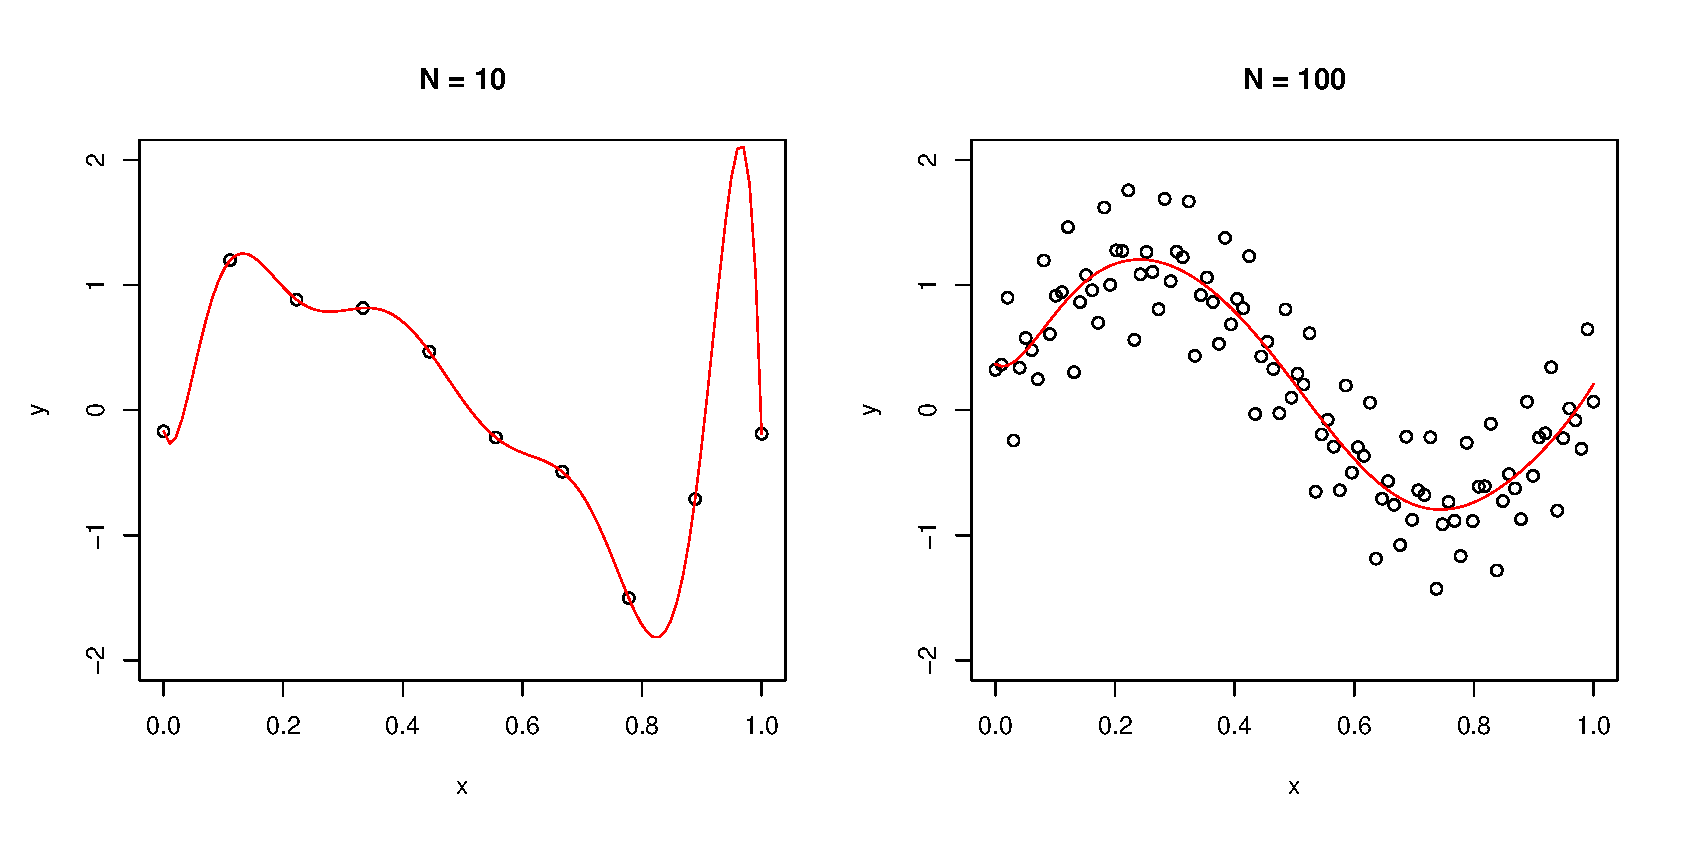
\includegraphics[height=2in]{02Background/bgPolyM9DataSizes.eps}
\end{center}
\caption{พหุนามดีกรี 9 ที่ฝึกกับชุดข้อมูลขนาดต่างกัน.
ภาพซ้ายฝึกกับข้อมูลขนาด $10$ จุดข้อมูล.
ภาพขวาฝึกกับข้อมูลขนาด $100$ จุดข้อมูล}
\label{fig: bg poly M9 different data sizes}
\end{figure}
%

\paragraph{เรกูลาไรเซชั่น.}
เรกูลาไรเซชั่น (Regularization) \index{regularization} \index{เรกูลาไรเซชั่น} 
เป็นวิธีหนึ่งที่นิยมใช้เพื่อช่วยลดปัญหาโอเวอร์ฟิตติ้ง.
แนวทางก็คือ การใส่\textit{พีนอลตี้เทอม} (Penalty Term) เข้าไปใน\textit{ฟังชั่นเป้าหมาย}
เพื่อจะถ่วงดุลไม่ให้ค่าสัมประสิทธิมีค่าใหญ่เกินไป.
สมการ~\ref{eq: bg regularization} แสดง\textit{ฟังชั่นเป้าหมาย}
ที่ประกอบด้วย\textit{ค่าผิดพลาด}และ\textit{พีนอลตี้เทอม} 
ซึ่งเป็นเทอมแรกและเทอมที่สองทางขวามือตามลำดับ.
%
นั่นคือ ฟังชั่นเป้าหมาย
\begin{eqnarray}
   \tilde{E}(\mathbf{w}) &=& \frac{1}{2} \sum_{n=1}^N \{ y(x_n, \mathbf{w}) - t_n \}^2 + \frac{\lambda}{2} \| \mathbf{w} \|^2
\label{eq: bg regularization}
\end{eqnarray}
เมื่อ $\| \mathbf{w} \|^2 \equiv \mathbf{w}^T \mathbf{w} = w_0^2 + w_1^2 + \ldots + w_M^2$ และ พารามิเตอร์ $\lambda$ ควบคุมสมดุลย์ระหว่างอิทธิพลของค่าผิดพลาดจากการทำนายและอิทธิพลของพีนอลตี้เทอม.
%
จากมุมมองของการหาค่าน้อยที่สุด 
พารามิเตอร์ $\lambda$ อาจถูกเรียกเป็น \textit{ลากองจ์พารามิเตอร์} 
(Lagrange Parameter, ดูหัวข้อ~\ref{sec: regularization} เพิ่มเติม หรือเรื่อง Constrained Optimization ของชองและเซค\cite{ChongZak2ndEd}).
\index{Lagrange Parameter}
%
บิชอบ\cite{Bishop2006a} ชี้ว่า บ่อยครั้งที่ \textit{พีนอลตี้เทอม}จะไม่รวม $w_0$ 
(นั่นคือ ใช้ $\sum_{i=1}^M w_i^2$ แทน $\| \mathbf{w} \|^2$).
หรือ ถ้ามี $w_0$ ก็อาจจะมีพารามิเตอร์ควบคุมอิทธิพลเฉพาะของตัวเอง.

รูป~\ref{fig: bg poly M9 reg different lambdas} แสดงผลจากเรกูลาไรเซชั่น จากลากองจ์พารามิเตอร์ค่าต่างๆ.
ภาพซ้ายสุด $\lambda = 0$ เทียบเท่ากับการไม่ได้ใช้พีนอลตี้เทอมเลย.
โอเวอร์ฟิตติ้งเห็นได้ชัดในกรณีนี้.
ภาพกลางแสดงค่าลากองจ์พารามิเตอร์ที่เหมาะสม 
ค่าลากองจ์พารามิเตอร์ที่เหมาะสมจะช่วยบังคับโมเดลที่มีความซับซ้อนสูงให้ทำตัวเหมือนกับโมเดลความซับซ้อนต่ำลง.
ค่าประมาณจากโมเดลแสดงด้วยเส้นทึบสีแดง มีลักษณะใกล้เคียงกับ $\sin(2 \pi x)$ ที่ใช้สร้างจุดข้อมูล.
แต่ถ้าหากใช้ค่าลากองจ์พารามิเตอร์มากเกินไป ก็อาจทำให้เกิด\textit{อันเดอร์ฟิตติ้ง} (Underfitting) ได้ดังแสดงในภาพขวาสุด.

เทียบกับตาราง~\ref{tbl: bg polynomial coeff} 
ตาราง~\ref{tbl: bg polynomial coeff regularization} แสดงให้เห็นว่า
ถ้าใช้ค่า $\lambda$ ใหญ่พอดี
เรกูลาไรเซชั่นช่วยควบคุมให้ค่าสัมประสิทธิไม่ใหญ่เกินไปได้.
แต่ถ้าใช้ค่า $\lambda$ ใหญ่เกินไป 
ก็ทำให้ค่าสัมประสิทธิน้อยเกินไปได้ เช่นกัน.
รูป~\ref{fig: bg poly regularization evaluation} แสดงผลค่าผิดพลาดของโมเดลพหุนามดีกรี 9 กับเรกูลาไรเซชั่นที่ค่าลากองจ์ต่างๆ 
เมื่อประเมินกับข้อมูลชุดฝึกหัดและชุดทดสอบ.
สังเกตุค่าผิดพลาดของโมเดล 
เมื่อประเมินกับชุดฝึกหัด ค่าผิดพลาดของโมเดลจะน้อยลง เมื่อใช้ค่าลากองจ์พารามิเตอร์น้อยๆ (ให้ผลคล้ายกับการใช้ฟังชั่นพหุนามดีกรีสูงๆ).
ส่วนเมื่อประเมินกับชุดทดสอบ ค่าผิดพลาดของโมเดลจะต่ำสุดที่ค่าลากองจ์ราวๆ $0.001$ หรือ $\log(\lambda) \approx -6.91$.

\begin{table}[hbtp]
\caption{ค่าสัมประสิทธิของพหุนามกับเรกูลาไรเซชั่นที่ลากองจ์พารามิเตอร์ค่าต่างๆ}
\begin{center}
\begin{tabular}{|c|r|r|r|}
\hline 
%
สัมประสิทธิ & $\lambda = 0$ & $\lambda = 10^{-5}$ & $\lambda = 1$ \\
\hline
$w_0$ & -0.17  & -0.04  & 0.5  \\
$w_1$ & -18.6  & 11.85  & -0.47  \\
$w_2$ & 1009.96  & -38.18  & -0.49  \\
$w_3$ & -11723.66  & 37.64  & -0.35  \\ 
$w_4$ & 64085.01  & -7.29  & -0.2  \\
$w_5$ & -195203.42  & -20.61  & -0.07  \\
$w_6$ & 349413.48  & -0.2  & 0.02  \\
$w_7$ & -365010.66  & 20.7  & 0.1  \\
$w_8$ & 205750.66  & 17.33  & 0.16  \\ 
$w_9$ & -48302.79  & -21.36  & 0.21  \\ 
%
\hline 
\end{tabular} 
\end{center}
\label{tbl: bg polynomial coeff regularization}
\end{table}


%
\begin{figure}
\begin{center}
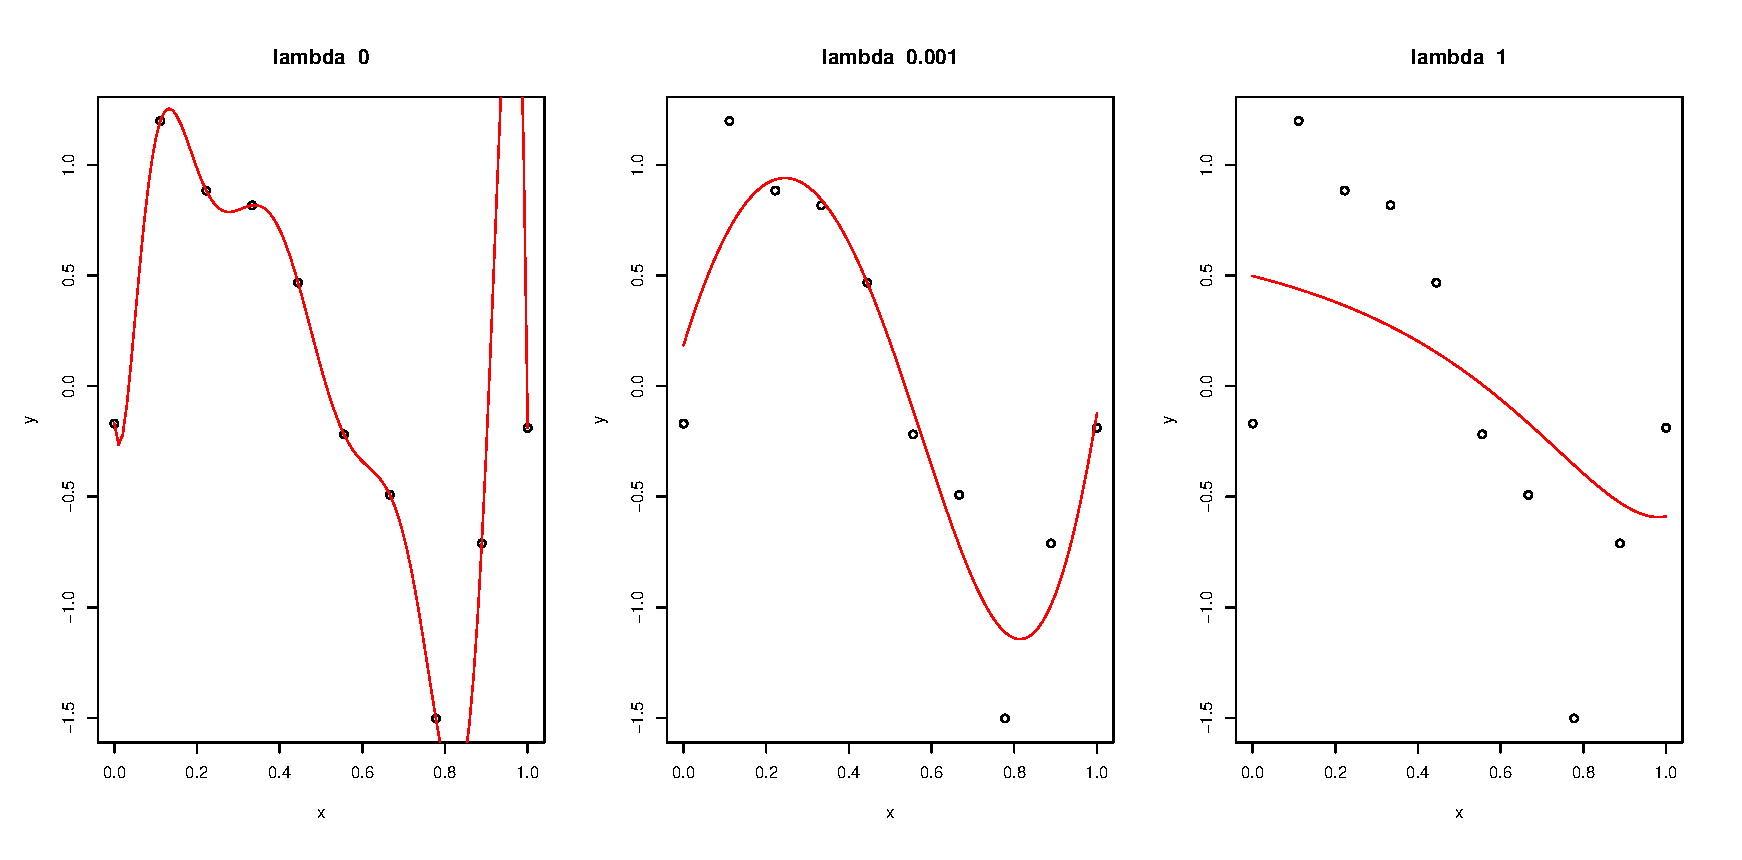
\includegraphics[height=2in]{02Background/bgPolyM9regLambdas.eps}
\end{center}
\caption{พหุนามดีกรี 9 กับเรกูลาไรเซชั่นด้วยลากองจ์พารามิเตอร์ค่าต่างๆ.
ภาพซ้ายแสดงโอเวอร์ฟิตติ้ง ($\lambda = 0$).
ภาพกลางแสดงโมเดลที่เหมาะสม ($\lambda = 0.001$).
ภาพขวาแสดงอันเดอร์ฟิตติ้ง ($\lambda = 1$)}
\label{fig: bg poly M9 reg different lambdas}
\end{figure}
%

%
\begin{figure}
\begin{center}
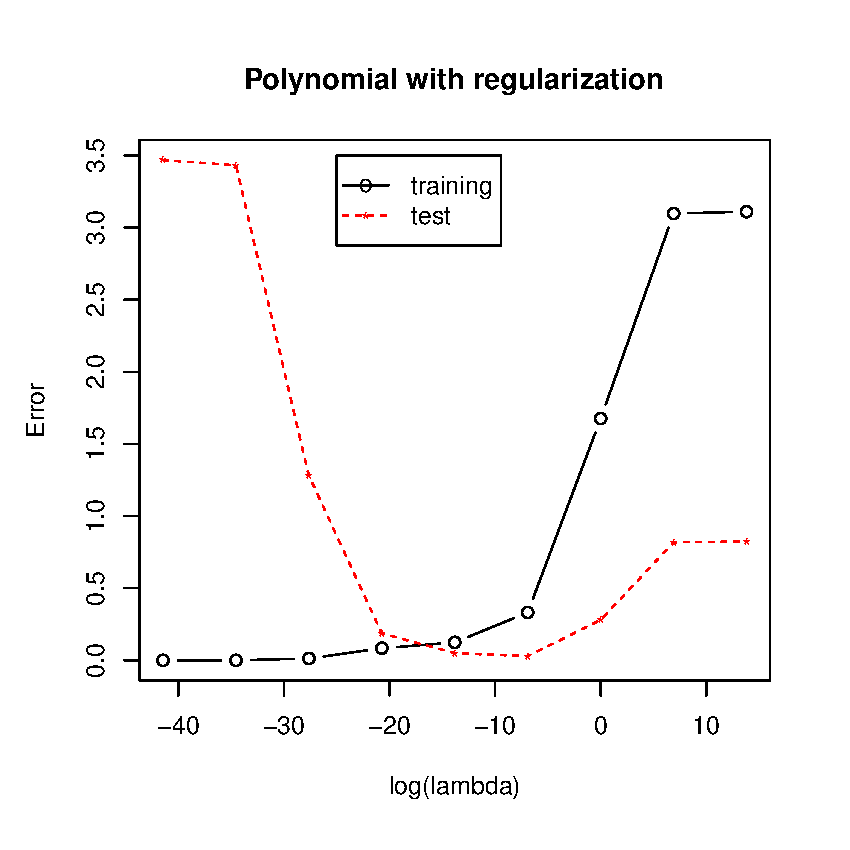
\includegraphics[height=2in]{02Background/bgPolyM9regTrainTest.eps}
\end{center}
\caption{เรกูลาไรเซชั่นด้วยลากองจ์พารามิเตอร์ค่าต่างๆ ประเมินด้วยข้อมูลชุดฝึกหัด กับ ชุดทดสอบ}
\label{fig: bg poly regularization evaluation}
\end{figure}
%

สำหรับการประเมินโมเดล สิ่งที่สำคัญคือคุณสมบัติที่โมเดลสามารถทำนายข้อมูลที่ไม่เคยเห็นมาก่อนได้ดี 
หรือเรียกว่า \textit{คุณสมบัติความทั่วไป} (Generalization). \index{generalization} \index{คุณสมบัติความทั่วไป}
เพื่อเลือกความซับซ้อนของโมเดล เช่น การเลือกดีกรีของพหุนาม หรือการเลือกค่าลากองจ์ของเรกูลาไรเซชั่น 
เราทำได้โดย การวัด\textit{คุณสมบัติความทั่วไป}ของโมเดลที่ความซับซ้อนต่างๆกัน.
วิธีง่ายๆและตรงไปตรงมาที่สุด ก็คือ การแบ่งข้อมูลออกเป็น $2$ ชุด
ได้แก่ \textit{ชุดที่ใช้ฝึกโมเดล} (Training Set) ที่ใช้หาค่าพารามิเตอร์ $\mathbf{w}$ 
และ\textit{ชุดวาลิเดชั่น} (Validation Set หรือ Hold-Out Set) \index{validation} \index{ข้อมูลชุดทำวาลิเดชั่น} ที่ใช้เลือกความซับซ้อนของโมเดล เช่น $M$ หรือ $\lambda$.

นอกจากนั้น เมื่อเลือกโมเดลได้แล้ว เพื่อทดสอบความสามารถของโมเดล เราควรจะมีข้อมูลที่แยกมาอีกชุดเพื่อทดสอบ 
เรียกว่า \textit{ชุดทดสอบ} (Test Set). \index{test set} \index{ข้อมูลชุดทดสอบ}
ที่ต้องมีชุดทดสอบนี้อีก เพื่อกันปัญหาที่เราอาจจะเลือกโมเดลที่เกิดโอเวอร์ฟิตติ้งกับชุดวาลิเดชั่น.
ถ้าเราเลือกโมเดลได้ดี ค่าผิดพลาดที่ประเมินกับข้อมูลชุดทดสอบไม่ควรห่างมากจากค่าผิดพลาดที่ประเมินกับข้อมูลชุดวาลิเดชั่น.

วิธีการเลือกโมเดลโดยการแบ่งบางส่วนของข้อมูลมาเป็นชุดวาลิเดชั่นนั้นเหมาะสมกับกรณีที่มีข้อมูลจำนวนมาก.
แต่หากข้อมูลมีขนาดจำกัด ผู้ทำโมเดลควรจะทำอย่างไร 
เมื่อการฝึกโมเดลให้ดีต้องการข้อมูลจำนวนมาก
และการทำวาลิเดชั่นที่ดีหรือการทดสอบที่ดีก็ต้องการข้อมูลจำนวนมากเช่นกัน.
การแบ่งส่วนข้อมูลที่ขนาดเล็กอยู่แล้ว ยิ่งจะทำให้แต่ละส่วนมีขนาดเล็กลงไปอีก.
วิธีหนึ่งที่ออกแบบมาเพื่อช่วยลดปัญหานี้ คือ \textit{วิธีครอสวาลิเดชั่น} (Cross-Validation). \index{cross-validation} \index{วิธีครอสวาลิเดชั่น}
แนวคิดคือ การฝึกโมเดลและการทำวาลิเดชั่นหลายๆครั้ง แล้วเอาผลมาเฉลี่ยกัน เพื่อหาโมเดลที่มี\textit{คุณสมบัติความทั่วไป}ดีที่สุด
โดยที่จะแบ่งข้อมูลออกเป็น $S$ ส่วน 
แต่ละครั้งจะเลือกส่วนหนึ่งมาเป็น\textit{ชุดวาลิเดชั่น}
และใช้ส่วนที่เหลือ ($S-1$ ส่วน) สำหรับฝึกโมเดล.
สำหรับ $S$ ส่วน จะเรียกว่า วิธีครอสวาลิเดชั้น $S$ พับ (S-Fold Cross-Validation).
วิธีครอสวาลิเดชั้น $S$ พับทำการฝึกและวาลิเดชั่น $S$ ครั้ง
ที่แต่ละครั้งจะใช้ส่วนที่ทำวาลิเดชั่นแตกต่างกัน.
เมื่อทำจนครบทุกส่วนแล้ว จึงนำค่าผิดพลาดที่ประเมินจากแต่ละครั้ง รวม $S$ ค่ามาหาค่าเฉลี่ย เป็น\textit{ค่าความผิดพลาดครอสวาลิเดชั่น}ของโมเดล (Cross-Validation Error).
\textit{ค่าความผิดพลาดครอสวาลิเดชั่น}นี้สามารถใช้เปรียบเทียบกับโมเดลอื่น (หรือโมเดลเดียวกันแต่ความซับซ้อนอื่น) เพื่อหาโมเดล(หรือความซับซ้อน)ที่ดีที่สุด.

%
\begin{figure}
\begin{center}
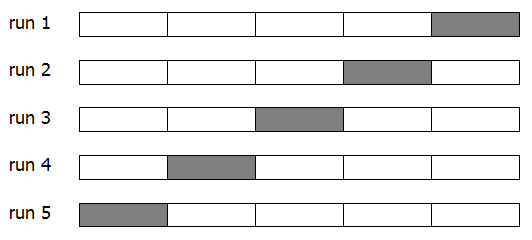
\includegraphics[height=2in]{02Background/crossvalidation.png}
\end{center}
\caption{วิธีครอสวาลิเดชั่น $5$ พับ. 
ข้อมูลทั้งหมดจะถูกแบ่งออกเป็น $5$ ส่วน 
และวิธีครอสวาลิเดชั่นจะทำทั้งหมด $5$ ครั้ง
โดยแผนภาพแสดงในเห็นว่า การทำครั้งแรกใช้ข้อมูล $4$ ส่วนแรกสำหรับการฝึก และส่วนสุดท้ายสำหรับวาลิเดชั่น.
ส่วนที่ใช้สำหรับวาลิเดชั่นจะแสดงเป็นสีเข้ม.
ครั้งที่สอง สาม สี่ และห้าก็ทำเช่นเดิม เพียงแต่เปลี่ยนส่วนที่มาทำวาลิเดชั่น.
}
\label{fig: bg cross validation}
\end{figure}
%

รูป~\ref{fig: bg cross validation} แสดงแผนภาพการแบ่งข้อมูลสำหรับวิธีครอสวาลิเดชั่น $5$ พับ ($S=5$) และการจัดสรรข้อมูลสำหรับการฝึกและการทำวาลิเดชั่นในแต่ละครั้ง. 
การฝึกและทำวาลิเดชั่นแต่ละครั้งจะเรียกเป็น\textit{วาลิเดชั่นรัน} (Validation Run).
ในภาพแสดง $5$ \textit{วาลิเดชั่นรัน} 
ที่รันแรก (Run 1) ฝึกโมเดลด้วยข้อมูล $4$ ส่วนแรก และโมเดลที่ฝึกแล้วไปทำวาลิเดชั่นกับส่วนหลังสุด (แรงเงาสีเข้มในรูป).
รันที่สองฝึกโมเดลด้วยข้อมูลส่วนอื่นยกเว้นส่วนที่ $4$ (แรงเงา) แล้วทำวาลิเดชั่นกับส่วนที่ $4$ ที่กันออกไว้.
ทำเช่นนี้จนครบ $5$ รัน แล้วนำเอาผลที่ได้มาเฉลี่ย.

ด้วยวิธีนี้ แต่ละรันจะฝึกโมเดลด้วยข้อมูลขนาด $S-1$ ของที่มีอยู่ 
และผลค่าผิดพลาดจากครอสวาลิเดชั่นก็เป็นค่าเฉลี่ยของค่าผิดพลาดที่ได้จากทุกส่วนของข้อมูล.
วิธีครอสวาลิเดชั่นนี้ทำให้เสมือนว่ามีข้อมูลมากขึ้น ทั้งการฝึกและการทำวาลิเดชั่น.
%ซึ่งเมื่อได้ผลเปรียบเทียบจากครอสวาลิเดชั่นแล้ว เราก็จะสามารถเลือกโมเดลได้จาก.

แม้วิธีครอสวาลิเดชั่นจะช่วยลดปัญหาของขนาดข้อมูลที่จำกัด และเป็นวิธีที่ใช้ข้อมูลได้อย่างคุ้มค่า
แต่ข้อเสียของวิธีครอสวาลิเดชั่นคือ การที่ต้องทำการรันทั้งหมด $S$ ครั้ง
โดยเฉพาะ หากถ้าการรันแต่ละครั้งใช้เวลามาก.
กล่าวอีกนัยก็คือ วิธีครอสวาลิเดชั่นใช้การคำนวณที่เพิ่มขึ้น เพื่อแก้ปัญหาข้อมูลขนาดเล็ก.
ดังนั้น หากถ้าการรันแต่ละครั้งใช้การคำนวณมากอยู่แล้ว แนวทางของวิธีครอสวาลิเดชั่นอาจจะไม่เหมาะสม
เช่น การฝึกโมเดลอาจจะมีการคำนวณสูง
หรือการทำครอสวาลิเดชั่นกับโมเดลที่มีพารามิเตอร์ที่ควบคุมความซับซ้อนหลายตัว
อาทิ การทำเรกูลาไรเซชั่นด้วยลากองจ์พารามิเตอร์หลายตัว อาจทำปริมาณการคำนวณเพิ่มขึ้นมหาศาล.

\paragraph{เกณฑ์สารสนเทศ.}

นอกจากแนวทางของวิธีวาลิเดชั่นที่ใช้ผลทดสอบกับข้อมูลชุดวาลิเดชั่นเป็นดัชนีบ่งชี้แล้ว
อีกแนวคิดหนึ่งก็คือการหาสูตรคำนวณที่ใช้ค่าประเมินผลกับข้อมูลชุดฝึกหัด รวมความซับซ้อนของโมเดลเข้าไปถ่วงดุลด้วย
โดยไม่ต้องทำวาลิเดชั่น.
แนวคิดนี้ ก็คือแนวทางของ\textit{เกณฑ์สารสนเทศ} (Information Criteria) \index{information criteria} \index{เกณฑ์สารสนเทศ}.
\textit{เกณฑ์สารสนเทศ} เป็นวิธีที่พยายามจะลดน้ำหนักผลประเมินที่ดีเกินไปกับข้อมูลชุดฝึกหัด(ที่อาจเกิดจากโอเวอร์ฟิตติ้ง)
ด้วยการใช้ความซับซ้อนของโมเดลเข้าไปถ่วงดุล เช่น \textit{เกณฑ์สารสนเทศอาไกอิเกะ}
(Akaike Information Criteria, คำย่อ AIC).

\textit{เกณฑ์สารสนเทศอาไกอิเกะ} คำนวณได้จาก
\index{Akaike Information Criteria} \index{เกณฑ์สารสนเทศอาไกอิเกะ}
%
\begin{eqnarray}
   \mathrm{AIC} = \ln p(\mathcal{D}|\mathbf{w}_{ML}) - M
\label{eq: AIC}.
\end{eqnarray}
โดย $p(\mathcal{D}|\mathbf{w}_{ML})$ คือ\textit{ลอการิทึ่มของค่าควรจะเป็นที่จัดแล้วพอดีที่สุด} (Best-Fit Log Likelihood) หรือกล่าวง่ายๆคือค่าลอการิทึ่มของความน่าจะเป็นที่โมเดลของจะให้ค่าเหมือนกับข้อมูลฝึกหัดเมื่อใช้\textit{ค่าพารามิเตอร์ที่ดีที่สุด} ($\mathbf{w}_{ML}$) 
และ $M$ คือจำนวนพารามิเตอร์ของโมเดล.

ค่า\textit{เกณฑ์สารสนเทศอาไกอิเกะ} $\mathrm{AIC}$ นี้ยิ่งมาก หมายถึงโมเดลยิ่งดียิ่งเหมาะสม.
%
ข้อดีของการใช้สูตรนี้ในการเลือกโมเดลคือเราแค่ทำการฝึกโมเดลอย่างเดียว ไม่ต้องทำวาลิเดชั่น 
ดังนั้นจึงไม่ต้องแบ่งข้อมูลไว้สำหรับวาลิเดชั่นและยังตัดขั้นตอนการทำวาลิเดชั่นลงไปได้ด้วย.
อย่างไรก็ตาม บิชอบ\cite{Bishop2006a} ได้ชี้ว่า ในทางปฏิบัติ 
สูตรลักษณะแบบนี้มักจะลำเอียงไปเลือกโมเดลที่ซับซ้อนน้อยเกินไป.
%วิธีที่ตรงไปตรงมาและเชื่อถือได้ที่สุดในการเลือกโมเดล คือ การทำวาลิเดชั่น.

\section{ความน่าจะเป็น}
\label{sec: Probability}
\index{probability} \index{ความน่าจะเป็น}

ปัจจัยหลักเรื่องหนึ่งสำหรับวิชาการเรียนรู้ของเครื่องและการรู้จำรูปแบบ ก็คือความไม่แน่นอน (Uncertainty).
ความไม่แน่นอนอาจจะมาจากหลายสาเหตุ เช่น ความไม่เที่ยงของเครื่องมือ หรือวิธีการวัด หรือวิธีการเก็บข้อมูล, สัญญาณรบกวน, ขนาดของข้อมูลที่จำกัด, หรือแม้แต่ธรรมชาติความหลากหลายและความแปรผันของข้อมูลเอง.
\textit{ทฤษฎีความน่าจะเป็น} (Probability Theory) 
เป็นแนวทางหนึ่งที่ให้กรอบวิธีการสำหรับการวัดและการจัดการกับความไม่แน่นอน 
และยังเป็นพื้นฐานที่สำคัญสำหรับการเรียนรู้ของเครื่อง.

\subsection{เซต}
\label{sec: sets}
\index{set} \index{เซต}

\textit{รูปแบบ} (Pattern) ที่เราสนใจ เช่น ลักษณะของรูปช้าง, สัญญาณเสียงของคำว่า ``ค้นหา'' เพื่อระบบสั่งงานด้วยเสียง, ลักษณะสำคัญของเอกสาร ที่บอกว่าเป็นเอกสารเกี่ยวกับข่าวกีฬา,
ลักษณะสำคัญของดอกไม้ที่ใช้ระบุได้ว่าเป็นดอกไม้พันธ์ุหิรัญญิกา เป็นต้น.
ทฤษฎีความน่าจะเป็นจะมอง\textit{รูปแบบ}เหล่านี้เป็นเหตุการณ์ เช่น เหตุการณ์ที่รูปที่สนใจเป็นภาพของช้าง, เหตุการณ์ที่สัญญาณเสียงที่ได้มาเป็นเสียงของคำว่า ``ค้นหา'' เป็นต้น.

\textit{เซต}แทนกลุ่มของ\textit{รูปแบบ}หรือ\textit{เหตุการณ์}ที่เราสนใจ เช่น เซตของรูปช้างแบบต่างๆ, เซตของเสียงคำว่า ``ค้นหา'' ที่น้ำเสียง สำเนียง ต่างๆ, 
เซตของอักขระในภาษาไทย, เป็นต้น.
ตาราง~\ref{tbl: prop set jargon}\footnote{
ดัดแปลงจาก ตาราง 1.1 ของกริมเมตต์กับสเติรซาเกอร์\cite{GrimmettStirzaker2001a}.
} แทนสัญญลักษณ์และคำศัพท์ที่เกี่ยวข้องกับ\textit{เซต}และ\textit{ความน่าจะเป็น}ที่ใช้บ่อยๆ.

\begin{table}[hbtp]
{\scriptsize
\caption{ภาษาเฉพาะ% (jargon) 
ที่ใช้ในเรื่อง\textit{เซต}กับ\textit{เรื่องความน่าจะเป็น}}
\begin{center}
\begin{tabular}{lll}
\hline
สัญญลักษณ์ทั่วไป  & ภาษาเฉพาะในเรื่องเซต & ภาษาเฉพาะในเรื่องความน่าจะเป็น \\
\hline
$\Omega$  & กลุ่มของวัตถุ & ปริภูมิตัวอย่าง (Sample Space) \\

$\omega$  & สมาชิกของ $\Omega$ & เหตุการณ์พื้นฐาน หรือ\textit{รูปแบบ} \\
%Member of $\Omega$ & Elementary event, outcome \\

$A$       & เซตย่อย (Subset) ของ $\Omega$ & เหตุการ์ที่มี\textit{รูปแบบ}ใน $A$ \\
%Subset of $\Omega$ & Event that some outcome in $A$ occurs \\

$A^c$     & \textit{ส่วนเติมเต็ม} (Complement) ของ $A$ & เหตุการ์ที่ไม่มี\textit{รูปแบบ}ใน $A$ \\
%Complement of $A$ & Event that no outcome in $A$ occurs \\ 

$A \cap B$ & \textit{อินเตอร์เซกชัน} (Intersection) & เหตุการณ์ที่มี\textit{รูปแบบ}ทั้งใน $A$ และใน $B$ \\
%Both $A$ and $B$ \\

$A \cup B$ & \textit{ยูเนียน} (Union) & เหตุการณ์ที่มี\textit{รูปแบบ}ใน $A$ หรือใน $B$ หรือในทั้งคู่\\
%Either $A$ or $B$ or both \\

$A \setminus B$ & ผลต่าง (Difference) & เหตุการณ์ที่มี\textit{รูปแบบ}ใน $A$ แต่ไม่มี\textit{รูปแบบ}ใน $B$ \\
%$A$, but not $B$ \\

%$A \uptriangle B$ & Symmetric difference & Either $A$ or $B$, but not both \\

%$A \subseteq B$ & Inclusion & If $A$, then $B$ \\

$\emptyset$ & เซตว่าง (Empty Set) & เหตุการณ์ที่เป็นไปไม่ได้ \\
%Impossible event \\

\hline
 \end{tabular} 
\end{center}
\label{tbl: prop set jargon}
}%end \small
\end{table}

\subsection{ความน่าจะเป็น}
\label{sec: probability main}
\index{probability}
\index{ความน่าจะเป็น}

กล่าวง่ายๆแล้ว ความน่าจะเป็น (Probability) ก็คือโอกาสที่เหตุการณ์ที่สนใจจะเกิดขึ้น.
นั่นคือ หากสมมติว่าเราทำการทดลองซ้ำๆเป็นจำนวน $N$ ครั้ง 
โดยให้สภาพแวดล้อมเหมือนเดิมมากเท่าที่จะเป็นไปได้.
กำหนดให้ $A$ เป็นเหตุการณ์ที่เราสนใจ 
โดย $A$ อาจจะเกิดขึ้นหรือไม่เกิดในแต่ละการทำซ้ำก็ได้.
สิ่งที่เราจะพบคือ
เมื่อจำนวนทำซ้ำ $N$ ใหญ่มากและใหญ่ขึ้นๆเป็นลำดับ
อัตราส่วนของจำนวนครั้งที่จะเกิด $A$ ในแต่ละการทำซ้ำ จะเข้าสู่ค่าๆหนึ่ง ซึ่งค่านั้นคือค่าความน่าจะเป็นของ $A$.

ขยายความคือ
หากกำหนดให้ $N(A)$ แทนจำนวนครั้งที่จะเกิดเหตุการณ์ $A$ ในการทำซ้ำทั้งหมด $N$ ครั้ง
อัตราส่วน $\frac{N(A)}{N}$ จะค่อยๆลู่เข้าสู่ค่าๆหนึ่ง เมื่อ $N$ เพิ่มขึ้น.
ค่าๆนั้นของอัตราส่วนจะเรียกว่า \textit{ความน่าจะเป็น}ที่เหตุการณ์ $A$ จะเกิดขึ้น ในแต่ละการทำซ้ำ
โดยค่าความน่าจะเป็นนี้ แทนด้วยสัญญลักษณ์ $\mathbb{P}(A)$.


หาก $A$ เป็นเหตุการณ์ที่เป็นไปไม่ได้, $A = \emptyset$, ดังนั้น $N(\emptyset) = 0$ และ $\mathbb{P}(A) = 0$.
ในทางกลับกัน หาก $A$ พูดถึงทุกๆเหตุการณ์ที่เป็นไปได้ $A = \Omega$, ดังนั้น $\mathbb{P}(A) = 1$.
ค่าของความน่าจะเป็น จะอยู่ระหว่าง $[0,1]$.
ตัวอย่างเช่น สมมติมีกล่องใส่ลูกบอลสีต่างๆ ดังแสดงในรูป~\ref{fig: prob red box} หากเราสุ่มหยิบลูกบอล ออกมาจากกล่อง $1$ ลูก,
ให้ $A$ เป็นเหตุการณ์ที่เราหยิบได้ลูกบอลสีเขียว.
สมมติเราทำการทดลอง(สุ่มหยิบ)ซ้ำ $N = 10$ เราได้ผลดังแสดงในรูป~\ref{fig: prob red box result N 10}
ซึ่งบอกได้ว่า อัตราส่วนที่หยิบได้ลูกบอลสีเขียว เป็น $\frac{N(A)}{N} = \frac{8}{10} = 0.8$.
หากเราเพิ่มจำนวนการทำซ้ำ $N$ จาก $10$ เป็น $100$, $1000$, $10000$, ...
เราจะเริ่มเห็นว่าอัตราส่วน $\frac{N(A)}{N}$ ลู่เข้าสู่ค่าๆหนึ่ง, ดังแสดงในตาราง~\ref{tbl: prob demo N(A)/N}.
เมื่อนำค่าต่างๆไปพล๊อตกราฟ จะได้ดังรูป~\ref{fig: prob demo N(A)/N} ซึ่งจะเห็นว่าค่าที่ อัตราส่วน $\frac{N(A)}{N}$ ลู่เข้าหาคือ $0.75$.
นั่นคือ ความน่าจะเป็นของการสุ่มหยิบได้ลูกเขียว, $\mathbb{P}(A) = 0.75$.
มองจากอีกมุมหนึ่ง ในกล่องมีลูกบอล $12$ และเป็นลูกสีเขียวอยู่ $9$ หากสุ่มหยิบด้วยความยุติธรรมแล้ว โอกาสที่จะหยิบได้ลูกเขียวก็น่าจะเป็น $\frac{9}{12} = 0.75$
ซึ่งค่าที่คำนวณนี้ก็สอดคล้องกับ\textit{ค่าความน่าจะเป็น}ที่ได้การทดลองข้างต้น.

%
\begin{figure}
\begin{center}
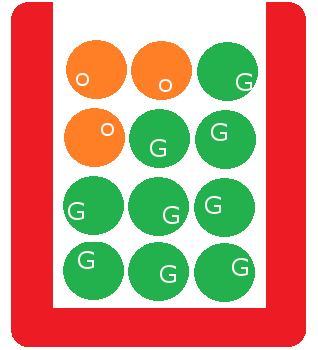
\includegraphics[width=2in]{02Prob/RedUrnMarked.png}
\end{center}
\caption{กล่องใส่ลูกบอล ซึ่งมีลูกบอลอยู่ภายใน $12$ ลูก เป็นลูกบอลสีส้มสามลูกและที่เหลือเป็นสีเขียว}
\label{fig: prob red box}
\end{figure}
%

%
\begin{figure}
\begin{center}
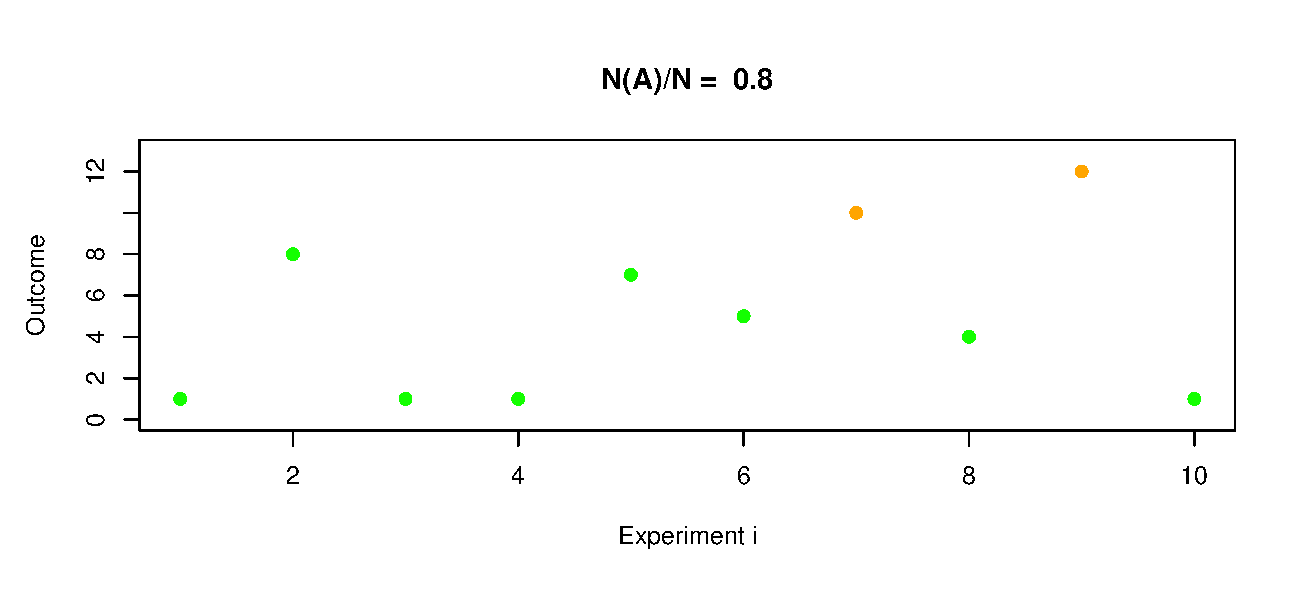
\includegraphics[width=4in]{02Prob/probDemo01.eps}
\end{center}
\caption{ผลจากการทดลองสุ่มหยิบลูกบอล $10$ ครั้ง จากกล่องลูกบอลที่แสดงในรูป~\ref{fig: prob red box}.
%  ในกล่องมีลูกบอล $12$ ลูก,
  ลูกที่ 1--9 สีเขียว ลูกที่ 10--12 สีส้ม.
  จากการสุ่มทำ $10$ ครั้ง มีครั้งที่ 7 และ 9 ที่หยิบได้ลูกบอลสีส้ม.
  ดังนั้น อัตราส่วนจำนวนครั้งที่หยิบได้ลูกบอลสีเขียว คือ $0.8$ (ระบุที่ด้านบนของภาพ)}
\label{fig: prob red box result N 10}
\end{figure}
%

\begin{table}[hbtp]
{\scriptsize
\caption{อัตราส่วนของการสุ่มได้ลูกบอลสีเขียว เมื่อจำนวนการทำซ้ำเพิ่มขึ้น}
\begin{center}
\begin{tabular}{|r|c|c|c|c|c|c|c|}
\hline 
$N$ & $10$ & $100$ & $1000$ & $10^4$ & $10^5$ & $10^6$ & $10^7$ \\
\hline 
$\frac{N(A)}{N}$ &
      $0.8$  & $0.68$  & $0.754$  & $0.7564$ & $0.74917$ & $0.749291$ &  $0.7499472$ \\
\hline
\end{tabular} 
\end{center}
\label{tbl: prob demo N(A)/N}
}%end \small
\end{table}

%
\begin{figure}
\begin{center}
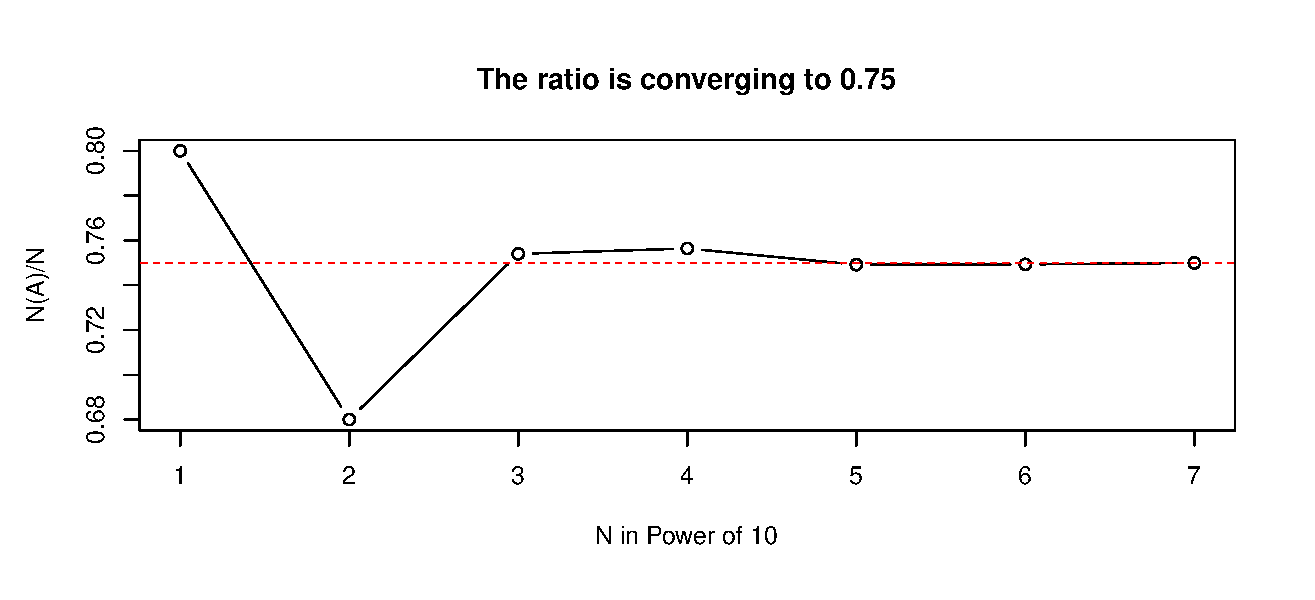
\includegraphics[width=4in]{02Prob/demoProb02.eps}
\end{center}
\caption{อัตราส่วน $\frac{N(A)}{N}$ ลู่เข้าหา $\mathbb{P}(A) = 0.75$ เมื่อ $N$ เพิ่มขึ้น (แสดงด้วยเส้นประสีแดง)}
\label{fig: prob demo N(A)/N}
\end{figure}
%

%
\begin{figure}
\begin{center}

\begin{tabular}{cc}
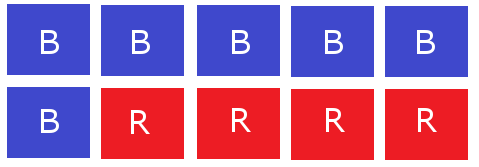
\includegraphics[width=2in]{02Prob/boxesMarked.png}
&
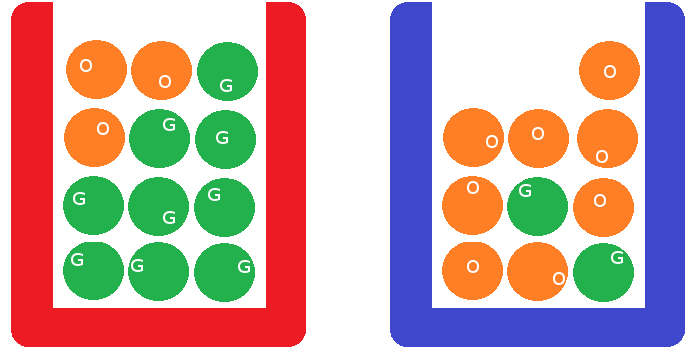
\includegraphics[width=2in]{02Prob/TwoUrnsMarked.png}
\\
(a) & (b) \\
\end{tabular} 
\end{center}
\caption{ตัวอย่างกล่องสีบรรจุลูกบอลสี สำหรับอภิปรายพื้นฐานเรื่องความน่าจะเป็นแบบมีเงื่อนไข.
ภาพ (a) แสดงสัดส่วนของกล่องสีฟ้ากับกล่องสีแดง (มีกล่องสีแดงอยู่ $4$ กล่อง ที่เหลือเป็นสีฟ้า).
ภาพ (b) แสดงสัดส่วนของลูกบอลสีภายในกล่องสองกล่อง โดย
กล่องซ้ายสีแดงมีลูกบอลสีส้มอยู่ $3$ ลูก ที่เหลือสีเขียว
และกล่องขวาสีฟ้ามีลูกบอลสีเขียวอยู่ $2$ ลูก ที่เหลือสีส้ม}
\label{fig: prob boxes}
\end{figure}
%

\paragraph{ความน่าจะเป็นมีเงื่อนไข (Conditional Probability).} 
\index{conditional probability}
\index{ความน่าจะเป็นมีเงื่อนไข}

จากตัวอย่างของรูป~\ref{fig: prob red box} 
ลองดูอีกตัวอย่างที่คราวนี้มีกล่อง $2$ แบบ กล่องสีแดง และ กล่องสีน้ำเงิน ดังรูป~\ref{fig: prob boxes}.
สมมติว่ากล่องที่จะได้ก็ถูกสุ่มมา 
และโอกาสที่จะสุ่มได้กล่องแดงเป็น $\frac{4}{10}$ หรือความน่าจะเป็นที่จะได้กล่องสีแดง $\mathbb{P}(C = \mbox{`r'}) = 0.4$,
โดย $C = \mbox{`r'}$ แทนเหตุการณ์ที่จะได้กล่องสีแดง.
ในทำนองเดียวกัน ความน่าจะเป็นที่จะได้กล่องสีฟ้า $\mathbb{P}(C = \mbox{`b'}) = 0.6$.

หากเรารู้แล้วว่าเป็นกล่องสีแดง เมื่อสุ่มหยิบลูกบอลมา เราก็รู้ว่าโอกาสที่จะหยิบได้ลูกบอลสีเขียว คือ $\frac{9}{12} = 0.75$ 
หรือกล่าวได้ว่า ความน่าจะเป็นที่จะหยิบได้ลูกบอลสีเขียวเมื่อหยิบจากกล่องสีแดง $\mathbb{P}(B = \mbox{`g'}|C = \mbox{`r'}) = 0.75$
โดย $B = \mbox{`g'}$ แทนเหตุการณ์ที่จะหยิบได้ลูกบอลเป็นสีเขียว.
ทำนองเดียวกัน ก็จะได้\textit{ความน่าจะเป็นมีเงื่อนไข}อื่นๆ (Conditional Probabilities) ดังนี้
\begin{itemize}
\item $\mathbb{P}(B = \mbox{`o'}|C = \mbox{`r'}) = 0.25$,
\item $\mathbb{P}(B = \mbox{`g'}|C = \mbox{`b'}) = 0.20$, 
\item $\mathbb{P}(B = \mbox{`o'}|C = \mbox{`b'}) = 0.80$.
\end{itemize}

สังเกตุว่า \textit{ความน่าจะเป็นที่จะหยิบได้ลูกบอลสีเขียวเมื่อรู้ว่าเป็นกล่องสีแดง} $\mathbb{P}(B = \mbox{`g'}|C = \mbox{`r'})$ ไม่เหมือนกับ\textit{ความน่าจะเป็นที่จะหยิบลูกบอลสีเขียวและได้กล่องสีแดง} $\mathbb{P}(B = \mbox{`g'}, C = \mbox{`r'})$.
สำหรับ\textit{ความน่าจะเป็นที่จะหยิบลูกบอลสีเขียวเมื่อรู้ว่าเป็นกล่องสีแดง} 
เราไม่ต้องสนใจเลยว่าโอกาสที่จะได้กล่องสีแดงเป็นอย่างไร.
ในขณะที่ \textit{ความน่าจะเป็นที่จะหยิบลูกบอลสีเขียวและได้กล่องสีแดง}จะประกอบด้วยโอกาสที่จะได้กล่องสีแดง $\mathbb{P}(C = \mbox{`r'})$ และโอกาสที่จะหยิบได้ลูกบอลสีเขียวจากกล่องนั้น $\mathbb{P}(B = \mbox{`g'}|C = \mbox{`r'})$
ซึ่งเขียนเป็นสมการได้
\begin{eqnarray}
  \mathbb{P}(B = \mbox{`g'}, C = \mbox{`r'}) &=& \mathbb{P}(C = \mbox{`r'}) \cdot \mathbb{P}(B = \mbox{`g'}|C = \mbox{`r'})
\label{eq: prob cond prob Balls and Crates} \\
  &=& (0.4) \cdot (0.75) = 0.3
\nonumber .
\end{eqnarray}

ในทำนองเดียวกันก็จะได้ว่า
\begin{itemize}
\item ความน่าจะเป็นที่จะหยิบได้ลูกบอลสีส้มและได้กล่องสีแดง
\\(หรือกล่าวอีกอย่างคือ ความน่าจะเป็นที่จะได้กล่องสีแดงและหยิบได้ลูกบอลสีส้ม)
\begin{eqnarray}
\mathbb{P}(B = \mbox{`o'},C = \mbox{`r'})
&=& \mathbb{P}(C = \mbox{`r'},B = \mbox{`o'})
\nonumber \\
&=& (0.4) \cdot (0.25) = 0.1
\nonumber ,
\end{eqnarray}
\item ความน่าจะเป็นที่จะหยิบได้ลูกบอลสีเขียวและได้กล่องสีฟ้า, $\mathbb{P}(B = \mbox{`g'},C = \mbox{`b'}) = (0.6) \cdot (0.2) = 0.12$,
\item ความน่าจะเป็นที่จะหยิบได้ลูกบอลสีส้มและได้กล่องสีฟ้า, $\mathbb{P}(B = \mbox{`o'},C = \mbox{`b'}) = (0.6) \cdot (0.8) = 0.48$.
\end{itemize}

ตาราง~\ref{tbl: prob cond prob table} สรุปค่าความน่าจะเป็นเหล่านี้.
สังเกตุประเด็นใหญ่ $3$ ประเด็น ดังนี้
ประเด็นที่ 1 ผลรวมของความน่าจะเป็นของทุกๆเหตุการณ์เป็น $1$. 
นั่นคือ
\begin{eqnarray}
\mathbb{P}(\Omega) &=& \mathbb{P}(C = \mbox{`r'}, B = \mbox{`g'})
  + \mathbb{P}(C = \mbox{`r'}, B = \mbox{`o'})
\nonumber \\
&\;&  
  + \mathbb{P}(C = \mbox{`b'}, B = \mbox{`g'})
  + \mathbb{P}(C = \mbox{`b'}, B = \mbox{`o'})    
\nonumber \\
&=& 0.3 + 0.1 + 0.12 + 0.48 = 1
\nonumber .
\end{eqnarray}
ธรรมชาตินี้เป็นคุณสมบัติพื้นฐานของความน่าจะเป็น.

ประเด็นที่ 2 ความน่าจะเป็นของเหตุการณ์ $X$ เท่ากับผลรวมของความน่าจะเป็นของเหตุการณ์ $X$ และ $Y$ สำหรับทุกๆความเป็นไปได้ของ $Y$,
\begin{eqnarray}
  \mathbb{P}(C = \mbox{`r'}) &=& \mathbb{P}(C = \mbox{`r'}, B = \mbox{`g'}) + \mathbb{P}(C = \mbox{`r'}, B = \mbox{`o'})
\label{eq: prob sum rule C=r} \\
  &=& 0.3 + 0.1 = 0.4
\nonumber \\
  \mathbb{P}(C = \mbox{`b'}) &=& \mathbb{P}(C = \mbox{`b'}, B = \mbox{`g'}) + \mathbb{P}(C = \mbox{`b'}, B = \mbox{`o'})
\label{eq: prob sum rule C=b} \\
  &=& 0.12 + 0.48 = 0.6
\nonumber .
\end{eqnarray}
ข้อสังเกตุนี้บอกธรรมชาติที่เรียกว่า \textit{กฏการบวก} (Sum Rule) \index{sum rule}
\index{sum rule}
\begin{eqnarray}
  p(X) = \sum_Y p(X,Y)
\label{eq: prop sum rule}  
\end{eqnarray}
เมื่อ $p(X)$ แทนความน่าจะเป็นของเหตุการณ์ $X$ และ
$p(X,Y)$ แทนความน่าจะเป็นที่จะมีทั้งเหตุการณ์ $X$ และเหตุการณ์ $Y$. 

กฏของการบวกนอกจากจะใช้หาค่าความน่าจะเป็นของการได้กล่องสีแดงหรือค่าความน่าจะเป็นของการได้กล่องสีฟ้าแล้ว
ยังสามารถใช้หาความน่าจะเป็นของการได้ลูกบอลสีเขียวได้ โดยไม่สนใจกล่อง.
สมการ~\ref{eq: prob sum rule B=g} แสดงการใช้กฏของการบวกในการหาความน่าจะเป็นของการได้ลูกบอลสีเขียว.
ในทำนองเดียวกัน ความน่าจะเป็นของการได้ลูกบอลสีส้ม ก็หาได้ดังแสดงในสมการ~\ref{eq: prob sum rule B=o},
\begin{eqnarray}
  \mathbb{P}(B = \mbox{`g'}) &=& \mathbb{P}(C = \mbox{`r'}, B = \mbox{`g'}) + \mathbb{P}(C = \mbox{`b'}, B = \mbox{`g'})
\label{eq: prob sum rule B=g} \\
&=& 0.3 + 0.12 = 0.42
\nonumber \\
  \mathbb{P}(B = \mbox{`o'}) &=& \mathbb{P}(C = \mbox{`r'}, B = \mbox{`o'}) + \mathbb{P}(C = \mbox{`b'}, B = \mbox{`o'})
\label{eq: prob sum rule B=o} \\
&=& 0.1 + 0.48 = 0.58
\nonumber .
\end{eqnarray}
ตาราง~\ref{tbl: prob cond prob table} สรุปค่าความน่าจะเป็นของตัวอย่างลูกบอลสีกับกล่อง.

\begin{table}[hbtp]
%{\scriptsize
\caption{สรุปค่าความน่าจะเป็นของตัวอย่างลูกบอลสีกับกล่อง}
\begin{center}
\begin{tabular}{|c|l|l|}
\hline 
กล่อง, & \multicolumn{2}{c|}{ลูกบอล, $B$ } \\
    \cline{2-3}
$C$ & เขียว, `g' & ส้ม, `o' \\
\hline
แดง, `r' & 0.3 & 0.1 \\
\hline
ฟ้า, `g' & 0.12 & 0.48 \\
\hline
\end{tabular} 
\end{center}
\label{tbl: prob cond prob table}
%}%end \small
\end{table}

ประเด็นที่ 3 เมื่อพิจารณาความน่าจะเป็นมีเงื่อนไข เช่น
ความน่าจะเป็นที่หยิบได้ลูกบอลสีเขียวเมื่อรู้ว่ากล่องสีแดง, $\mathbb{P}(B = \mbox{`g'}|C = \mbox{`r'})$, ความหมายคือพิจารณาเฉพาะเวลาที่ได้กล่องเป็นสีแดงว่ามีโอกาสได้ลูกบอลสีเขียวเท่าไร หรือเขียนได้เป็น
\begin{eqnarray}
\mathbb{P}(B = \mbox{`g'}| C = \mbox{`r'}) &=& \lim_{N \rightarrow \infty} \frac{ N(B = \mbox{`g'}, C = \mbox{`r'}) }{ N(C = \mbox{`r'}) }
\nonumber \\
 &=& \lim_{N \rightarrow \infty} \frac{ N(B = \mbox{`g'}, C = \mbox{`r'}) }{N} \cdot \frac{N}{ N(C = \mbox{`r'}) }
\nonumber \\
 &=&  \mathbb{P}(B = \mbox{`g'}, C = \mbox{`r'}) \cdot \frac{1}{\mathbb{P}(C = \mbox{`r'})}
\label{eq: prob cond prob}  .
\end{eqnarray}
สมการ~\ref{eq: prob cond prob} สอดคล้องกับ สมการ~\ref{eq: prob cond prob Balls and Crates} ที่อภิปรายไปก่อนหน้า.
ความจริงข้อนี้สรุปออกมาเรียกว่า \textit{กฏของการคูณ} (Product Rule), 
\index{product rule}
\index{กฏของการคูณ}
นั่นคือ
\index{product rule}
\begin{eqnarray}
p(X,Y) = p(Y|X) \cdot p(X)
\label{eq: prob product rule} .
\end{eqnarray}

เพื่อความสะดวก ความน่าจะเป็นของ $X$ และ $Y$ หรือ $p(X,Y)$ อาจจะถูกเรียกว่า \textit{ความน่าจะเป็นร่วม} (Joint Probability).
\index{ความน่าจะเป็นร่วม}
\index{joint probability}
เทอม $p(Y|X)$ เป็น\textit{ความน่าจะเป็นมีเงื่อนไข} (Conditional Probability)
%, อ่าน probability of $Y$ given $X$,
และ $p(X)$ บางครั้งจะเรียกว่า \textit{ความน่าจะเป็นตามขอบ} (Marginal Probability).
\index{marginal probability}
\index{ความน่าจะเป็นตามขอบ}

กฏของการบวกสามารถใช้คำนวณย้อยกลับได้ว่า ถ้าลูกบอลที่ได้สีเขียว มีโอกาสมากเท่าไรที่มันจะถูกหยิบมาจากกล่องสีแดง
หรือ ความน่าจะเป็นของการได้กล่องสีแดงเมื่อรู้ว่าหยิบได้ลูกบอลสีเขียว
% (probability that the box is red given the ball is green),
\begin{eqnarray}
\mathbb{P}(C = \mbox{`r'}|B &=& \mbox{`g'}) = \frac{\mathbb{P}(C = \mbox{`r'},B = \mbox{`g'})}{\mathbb{P}(B = \mbox{`g'})}
\label{eq: prop P(C|B) origin} 
\end{eqnarray}
และจากกฏของการบวก จะได้ว่า
\begin{eqnarray}
\mathbb{P}(B = \mbox{`g'}) &=&
  \sum_{c \in \{\mbox{`r'}, \mbox{`b'}\} } \mathbb{P}(C=c,B = \mbox{`g'})
\nonumber 
\end{eqnarray}
ดังนั้น
\begin{eqnarray}
\mathbb{P}(C = \mbox{`r'}|B &=& \mbox{`g'}) = \frac{\mathbb{P}(C = \mbox{`r'},B = \mbox{`g'})}{\sum_c \mathbb{P}(C=c,B = \mbox{`g'})}
\label{eq: prob P(C|B) 1} \\
&=& \frac{0.3}{0.3 + 0.12} = \frac{0.3}{0.42} \approx 0.71
\nonumber .
\end{eqnarray}
นอกจากนั้น 
สมการ~\ref{eq: prop P(C|B) origin} ช่วยเพิ่มแนวทางที่สามารถคำนวณไปในแนวอื่นอีกได้ เช่น
\begin{eqnarray}
\mathbb{P}(C = \mbox{`r'}|B &=& \mbox{`g'}) = \frac{\mathbb{P}(B = \mbox{`g'}|C = \mbox{`r'}) \cdot \mathbb{P}(C = \mbox{`r'})}{\mathbb{P}(B = \mbox{`g'})}
\label{eq: prop P(C|B) 2} 
\end{eqnarray}
ซึ่งเรารู้ว่า $\mathbb{P}(B = \mbox{`g'}|C = \mbox{`r'}) = 0.75$, 
$\mathbb{P}(C = \mbox{`r'}) = 0.4$ และ $\mathbb{P}(B = \mbox{`g'}) =0.42$ (จากสมการ~\ref{eq: prob sum rule B=g}), ดังนั้นก็จะรู้ว่า
$\mathbb{P}(C = \mbox{`r'}|B = \mbox{`g'}) = (0.75 \cdot 0.4)/0.42 \approx 0.71$, ซึ่งก็สอดคล้องกับผลก่อนหน้าที่แสดงในสมการ~\ref{eq: prob P(C|B) 1}.

\subsection{ตัวอย่างปัญหาความน่าจะเป็นมีเงื่อนไข}

ตัวอย่างหนึ่งที่แสดงผลของการใช้งาน\textit{ความน่าจะเป็นแบบมีเงื่อนไข}ได้เป็นอย่างดี 
คือตัวอย่างปัญหามอนตี้ฮอล (Monty Hall Problem).
\index{ปัญหามอนตี้ฮอล} \index{Monty Hall Problem}
สถานะการณ์คือ สมมติว่าคุณบัวผุดได้ไปเล่นเกมส์โชว์ ที่คุณบัวผุดจะต้องเลือกเปิดประตูหนึ่งในสามประตู.
มีประตูหนึ่งที่ซ่อนหีบสมบัติรัตนมณีไว้.
อีกสองประตูซ่อนหีบขยะไว้.
หลังจากคุณบัวผุดเลือกประตูไปแล้ว แทนที่พิธีกรจะเปิดประตูนั้นออกทันที.
พิธีกรกลับเดินไปเปิดอีกประตูให้ดูว่ามีหีบขยะอยู่หลังประตูนั้น 
และเสนอโอกาสให้คุณบัวผุดจะเปลี่ยนใจไปเลือกประตูที่เหลืออยู่ ซึ่งเป็นประตูคุณบัวผุดไม่ได้เลือกแต่แรกและก็ยังไม่ถูกเปิด.
คุณบัวผุดควรจะเลือกยืนยันประตูเก่า หรือควรจะเลือกเปลี่ยนไปประตูใหม่?

ปัญหานี้ ในมุมมองของความน่าจะเป็นมีเงื่อนไขเท่ากับการหาค่าความน่าจะเป็นที่ประตูใหม่จะมีหีบสมบัติรัตนมณีอยู่ 
เมื่อรู้ว่าแล้วว่า ประตูหนึ่งถูกเลือกไปแล้วและอีกประตูหนึ่งถูกเปิดไปแล้ว
นั่นคือ การหา $\mathbb{P}(A = 3|C = 1, H = 2)$,
โดย ให้ $A = 3$ แทนการที่ประตูที่สามจะมีหีบสมบัติรัตนมณีอยู่
$C = 1$ แทนคุณบัวผุดเลือกประตูที่หนึ่ง 
$H = 2$ แทนพิธีกรเปิดประตูที่สองไปแล้ว.
หากรู้ว่าพิธีกรเปิดประตูที่สอง แล้ววิเคราะห์ดูจะพบว่า
\begin{itemize}
\item ถ้าหีบสมบัติรัตนมณีอยู่ประตูที่คุณบัวผุดเลือก พิธีกรมีโอกาสเลือกหนึ่งในสองประตูที่เหลือ.
ดังนั้นในกรณีนี้ โอกาสที่พิธีกรจะเปิดประตูที่สอง คือ
\\ $\mathbb{P}(H = 2| C = 1, A = 1) = 0.5$.
\item พิธีกรจะไม่เปิดประตูที่มีหีบสมบัติรัตนมณีอยู่.
ดังนั้นในกรณีที่หีบสมบัติรัตนมณีอยู่หลังประตูที่สอง โอกาสที่พิธีกรจะเปิดประตูที่สองคือ
\\ $\mathbb{P}(H = 2| C = 1, A = 2) = 0$.
\item ถ้าหีบสมบัติรัตนมณีไม่อยู่ประตูที่คุณบัวผุดเลือก พิธีกรต้องเปิดประตูเดียวที่เหลืออยู่.
ดังนั้น โอกาสคือ
\\ $\mathbb{P}(H = 2| C = 1, A = 3) = 1$.
\end{itemize}

จาก\textit{กฏของการคูณ} จะได้ว่า
\begin{eqnarray}
%  \mathbb{P}(A = 3|C = 1, H = 2) \cdot \mathbb{P}(H = 2, C = 1) 
%  &=& \mathbb{P}(A = 3, C = 1, H = 2)
%  \nonumber \\
%  =
%  \mathbb{P}(H = 2|C = 1, A = 3) \cdot \mathbb{P}(A = 3, C = 1) 
%\nonumber \\
\mathbb{P}(A = 3|C = 1, H = 2)
&=&
  \frac{\mathbb{P}(H = 2|C = 1, A = 3) \cdot \mathbb{P}(A = 3, C = 1) }{ \mathbb{P}(H = 2, C = 1) }
\nonumber
\end{eqnarray}
และเมื่อนับ จะได้ว่า $\mathbb{P}(A = 3, C = 1) = \frac{1}{9}$ เพราะว่า มีโอกาสเป็น $(A = 1, C = 1)$, $(A = 1, C = 2)$, $(A = 1, C = 3)$, $(A = 2, C = 1)$, ..., $(A = 3, C = 3)$ แต่ละอันเท่าๆกัน (มี $9$ แบบ เพราะฉะนั้น ก็ $1$ ใน $9$)
และจากกฏการบวก จะได้ว่า
\begin{eqnarray}
\mathbb{P}(H = 2, C = 1) &=& \mathbb{P}(H = 2, C = 1, A = 1) + \mathbb{P}(H = 2, C = 1, A = 2) 
\nonumber \\
  &\;& + \mathbb{P}(H = 2, C = 1, A = 3)
\nonumber \\
&=& \mathbb{P}(H = 2| C = 1, A = 1) \cdot \mathbb{P}(C = 1, A = 1)
\nonumber \\
&\;& + \mathbb{P}(H = 2| C = 1, A = 2)  \cdot \mathbb{P}(C = 1, A = 2)
\nonumber \\
  &\;& + \mathbb{P}(H = 2| C = 1, A = 3) \cdot \mathbb{P}(C = 1, A = 3)
\nonumber \\
&=& (0.5) \cdot \frac{1}{9} + (0) \cdot \frac{1}{9} + 1 \cdot \frac{1}{9} = \frac{1.5}{9}
\nonumber .
\end{eqnarray}
ดังนั้นก็จะได้
\begin{eqnarray}
\mathbb{P}(A = 3|C = 1, H = 2) &=& \frac{ \frac{1}{9} }{ \frac{1.5}{9} } = \frac{2}{3}
\nonumber .
\end{eqnarray}
ผลที่ได้บอกว่า เมื่อพิธีกรเสนอให้คุณบัวผุดเปลี่ยนประตู ถ้าคุณบัวผุดเปลี่ยน คุณบัวผุดมีโอกาสได้หีบสมบัติรัตนมณีเป็น 
$\frac{2}{3} \approx 66.7\%$.

เมื่อดูผลการคำนวณแล้ว หลายๆคนอาจไม่เชื่อและอาจคิดว่ามันเป็นแค่ผลจากทฤษฎี
ผู้เขียนจึงใช้โค้ดต่อไปนี้จำลองสถานะการณ์ให้เห็น
และผู้เขียนสนับสนุนให้ผู้อ่านที่สงสัยทดลองด้วยตนเอง.
%
โค้ดต่อไปนี้จำลองสถานะการณ์ทั้งหมด $N = 100$ ครั้ง
\begin{lstlisting}[language=R]
N = 100
doors = c(1,2,3)

recs = matrix(0, 3, N)
for(i in 1:N){
  ## which door has jewels
  jewels = sample(doors,1)

  ## which door has been chosen
  chosen = sample(doors,1)

  ## which door has the host opened
  open = sample( rep(doors[-c(jewels, chosen)],2), 1)

  recs[,i] = c(jewels, chosen, open)
}

## Count how many times Rising Lotus will get the jewels without switching
sum(recs[2,] == recs[1,])

## Count how many times Rising Lotus will get the jewels with switching
sum(recs[2,] != recs[1,])
\end{lstlisting}
สังเกตุว่า การจำลองประตูที่ซ่อนหีบสมบัติรัตนมณี \verb|jewels = sample(doors,1)| และ 
ประตูที่คุณบัวผุดเลือก \verb|chosen = sample(doors,1)| จะสุ่มตรงๆจากประตูที่มี.
แต่ประตูที่พิธีกรเลือกเปิดให้ดู พิธีกรจะเลือกเปิดได้เฉพาะประตูที่ไม่มีหีบสมบัติหรือไม่ถูกเลือก
ในโค้ดใช้ ดัชนี \verb|-c(jewels, chosen)| 
เพื่อตัด\textit{ประตูที่มีหีบสมบัติและประตูที่ถูกเลือก}ออกจากรายการประตูที่พิธีกรจะเลือกเปิดได้.
เมื่อนับจำนวนครั้งที่ประตูที่คุณบัวผุดเลือก (บันทึกไว้ใน \verb|recs[2,]|) ที่ตรงกับประตูที่มีหีบสมบัติ (บันทึกไว้ใน \verb|recs[1,]|) 
และเปรียบเทียบกับจำนวนครั้งที่ประตูที่คุณบัวผุดเลือกไม่ตรงกับประตูที่มีหีบสมบัติ แปลว่า ถ้าคุณบัวผุดเปลี่ยน คุณบัวผุดจะได้สมบัติรัตนมณี.
เมื่อทดลองด้วยตนเองแล้ว ผู้อ่านจะเห็นว่า ผลที่ได้จะสอดคล้องกับการคำนวณ $\mathbb{P}(A = 3|C = 1, H = 2) = \frac{2}{3}$ และผลจะยิ่งเห็นชัดขึ้น เมื่อลองให้จำนวนครั้ง $N$ เพิ่มขึ้น.

%%%%%%%%%%%%%%%%%%%%%%%%%%%%%%%%%%%%%%%%%%%%%%%%%%%%%%%%%%%%%%%%
\section{แบบฝึกหัด}
\label{section: bg exercises}

%\subsection{การหาค่าถดถอยด้วยฟังชั่นพหุนาม}

\paragraph{1.} จากตัวอย่างการพัฒนาที่มาของสมการฝึกฟังชั้นพหุนามอันดับหนึ่ง (ตั้งแต่สมการ~\ref{eq: bg polynomial derivatives 2a},
\ref{eq: bg polynomial derivatives 2b} 
ไปจนได้ สมการ~\ref{eq: bg polynomial M1})
จงหาสมการฝึกฟังชั้นพหุนามอันดับสองและอันดับสาม (เขียนเป็นเมตริกซ์แบบเดียวกับสมการ~\ref{eq: bg polynomial M1})

\paragraph{2.} จากตัวอย่างในกิจกรรมโปรแกรมหาค่าถดถอย 
จงเขียนฟังชั่นเพื่อคำนวณหาค่าพารามิเตอร์และค่าเอาท์พุต สำหรับฟังชั้นพหุนามอันดับสองและอันดับสาม (ดูตัวอย่าง \texttt{w.polyfit1} และ \texttt{y.poly1})

\paragraph{3.} สังเกตุสมการฝึกโมเดลฟังชั่นพหุนามอันดับ 2 และ 3 ที่ได้จากข้อ 1, จงหาสมการฝึกฟังชั้นพหุนามอันดับใดๆ $M$ โดยที่ $M$ อาจเป็นค่าใดๆ ตั้งแต่ 1 ขึ้นไป. 

\paragraph{4.} จากแบบฝึกหัดข้อ 3 
จงเขียนฟังชั่นเพื่อคำนวณหาค่าพารามิเตอร์และค่าเอาท์พุต สำหรับฟังชั่นพหุนามอันดับ $M$ โดย $M$ อาจเป็นค่าใดๆ ตั้งแต่ $1$ ขึ้นไป. 
ตัวอย่างเช่น อาจเรียกฟังชั่นด้วย \texttt{w <- w.polyfitM(dp.x, dp.t, M=8)}, \texttt{forecast.y <- y.poly(x, w)} เป็นต้น. 

\paragraph{5.} จากโปรแกรมที่เป็นคำตอบของแบบฝึกหัดข้อ 4
จงทดลองฝึกฟังชั่นพหุนามอันดับ 1, 2, 3, 4, 5, 6, 7, 8, และ 9 แล้วนำผลมาวาดภาพดังรูป~\ref{fig: bg ex 5}.

%
\begin{figure}
\begin{center}
\includegraphics[width=5.5in]{02Background/bgEx01.eps}
\end{center}
\caption{ภาพประกอบแบบฝึกหัดข้อ 5.
ผลจากโมเดลพหุนามอันดับ 1 ถึง 9 ที่ฝึกแล้ว (เส้นสีแดง)}
\label{fig: bg ex 5}
\end{figure}
%

\paragraph{6.} จากแบบฝึกหัดข้อ 5 
ถ้าหากทำข้อ 5 แล้วไม่ได้ผลดังรูป~\ref{fig: bg ex 5} 
แต่กลับได้ผลดังรูป~\ref{fig: bg ex 6}. 
จงอภิปรายว่าเกิดอะไรขึ้น และอภิปรายข้อดีข้อเสียเปรียบเทียบระหว่างการวาดภาพในแบบรูป~\ref{fig: bg ex 5} และรูป~\ref{fig: bg ex 6}.

%
\begin{figure}
\begin{center}
\includegraphics[width=5.5in]{02Background/bgEx06.eps}
\end{center}
\caption{ภาพประกอบแบบฝึกหัดข้อ 6.
ผลจากโมเดลพหุนามอันดับ 1 ถึง 9 ที่ฝึกแล้ว (เส้นสีแดง)}
\label{fig: bg ex 6}
\end{figure}
%

\paragraph{7.} จากแบบฝึกหัดข้อ 5
จงศึกษาผลที่ได้และอภิปรายว่า
ถ้าจะเลือกต้องเลือกโมเดลระหว่างฟังชั่นพหุนามอันดับที่ 1 ถึง 9 
ผู้ใช้ควรจะเลือกฟังชั่นพหุนามอันดับใด เพราะอะไร.

\paragraph{8.} จงวิเคราะห์โปรแกรมในแบบฝึกหัดข้อ 4 และทดลองฝึกโมเดลด้วยอันดับที่สูงกว่า 9 ว่าเป็นอย่างไร ถ้ารันไม่ได้ เป็นเพราะอะไร อภิปราย.
[\textbf{คำใบ้:} ถ้าโปรแกรมที่เขียนใช้ \texttt{solve} หรือวิธีการแก้สมการตรงๆ เพื่อหาค่า \texttt{w} ดังโค้ดตัวอย่างอันดับหนึ่งในหัวข้อ\ref{section: Polynomial Curve Fitting} แล้ว จะไม่สามารถแก้สมการได้ เมื่อจำนวนจุดข้อมูลน้อยกว่าจำนวนสัมประสิทธิ์. 
ศึกษาเพิ่มเติม\textit{พีชคณิตเชิงเส้น} (Linear Algebra).]

\paragraph{9.} ภายในฟังชั่น \texttt{w.polyfit1} หรือ \texttt{w.polyfitM} ให้ทดลองเปลี่ยนจากการแก้สมการด้วย \texttt{solve} เป็นการใช้วิธีลงเกรเดียนต์ (ดูหัวข้อ \ref{sec: Gradient Descent}) แล้วทดลองฝึกโมเดลด้วยอันดับต่างๆ ว่าเป็นอย่างไร เปรียบเทียบกับผลที่ได้กับคำตอบจากแบบฝึกหัดข้อ 7--8.

\paragraph{10.} \textit{การขยายของอนุกรมเทย์เลอร์} (Taylor Series Expansion) กล่าวว่า 
ถ้า $f(x)$ สามารถหาอนุพันธ์ได้ทุกๆอันดับไม่จำกัด (indefinitely differentiable) ที่ $x_0$ แล้ว
\begin{eqnarray}
   f(x) = f(x_0) + \frac{f'(x_0)}{1!}(x - x_0) + \frac{f''(x_0)}{2!}(x - x_0)^2  + \frac{f^{(3)}(x_0)}{3!}(x - x_0)^3 + \cdots.
\nonumber \\
\label{eq: Taylor}
\end{eqnarray}
\index{Taylor series} \index{อนุกรมเทย์เลอร์}
จาก\textit{การขยายของอนุกรมเทย์เลอร์} จงกระจายฟังชั่น $\sin(2 \pi x)$.

\paragraph{11.} จงนำสมการที่ได้จากข้อ 10 ไปเขียนโปรแกรมและวาดกราฟ 
โดยให้อนุกรมกระจายไปถึงดีกรี 1 ถึง 9 (วาด 9 ภาพ) 
และ (ก) ให้ $x_0 = 0$ กับ (ข) ให้ $x_0 = 0.5$, ดังตัวอย่างในรูป~\ref{fig: bg taylor}.
อภิปรายสิ่งที่ได้.

%
\begin{figure}
\begin{center}
\includegraphics[width=5.5in]{02Background/bgTaylorSine.eps}
\end{center}
\caption{ตัวอย่างภาพของการกระจายเทย์เลอร์.
เส้นทึบสีดำแสดงฟังชั่น $\sin(2 \pi x)$. 
เส้นประสีแดงแสดงการประมาณจากการกระจายเทย์เลอร์.
ภาพต่างๆทางซ้ายแสดงการกระจายเทย์เลอร์ที่ใช้ $x_0 = 0$.
ภาพต่างๆทางขวาแสดงการกระจายเทย์เลอร์ที่ใช้ $x_0 = 0.5$.
ดีกรีของการกระจายเทย์เลอร์ระบุอยู่ในแต่ละภาพ}
\label{fig: bg taylor}
\end{figure}
%

%\subsection{การเลือกโมเดล}

\paragraph{12.} จากตัวอย่างการพัฒนาจนได้สมการ~\ref{eq: bg polynomial M1} 
จงแสดงการหาสมการ~\ref{eq: bg w of reg poly deg 1},
\begin{eqnarray}
%
\left[ 
\begin{matrix}
N & \sum_{n=1}^N x_n \\
\sum_{n=1}^N x_n & (\sum_{n=1}^N x_n^2) + \lambda
\end{matrix}
\right] \cdot 
\left[ 
\begin{matrix}
w_0 \\
w_1
\end{matrix}
\right]
=
\left[ 
\begin{matrix}
\sum_{n=1}^N t_n \\
\sum_{n=1}^N t_n \cdot x_n
\end{matrix}
\right]
\label{eq: bg w of reg poly deg 1}
\end{eqnarray}
เมื่อใช้เรกูลาไรเซชั่นกับพหุนามดีกรีหนึ่ง,
\begin{eqnarray}
   \tilde{E}(\mathbf{w}) &=& \frac{1}{2} \sum_{n=1}^N \{ (w_0 + w_1 x_n) - t_n \}^2 + \frac{\lambda}{2} (w_1^2).
\label{eq: bg regularized polynomial degree 1 E}
\end{eqnarray}
สังเกตุ ไม่มีการทำเรกูลาไรเซชั่นกับ $w_0$.

\paragraph{13.} ในทำนองเดียวกับข้อ 12 สำหรับพหุนามดีกรีใดๆ $M$ กับ เรกูลาไรเซชั่น จงแสดงการหาสมการ~\ref{eq: bg w of reg poly deg M},
\begin{eqnarray}
%
\left[ 
\begin{matrix}
N & \sum_{n=1}^N x_n & \sum_{n=1}^N x_n^2 & \cdots &  \sum_{n=1}^N x_n^M \\
\sum_{n=1}^N x_n & \sum_{n=1}^N x_n^2 + \lambda & \sum_{n=1}^N x_n^3 & \cdots &  \sum_{n=1}^N x_n^{M+1} \\
\sum_{n=1}^N x_n^2 & \sum_{n=1}^N x_n^3 & \sum_{n=1}^N x_n^4  + \lambda & \cdots & \sum_{n=1}^N x_n^{M+2} \\
\vdots & \vdots & \vdots & \ddots & \vdots \\
\sum_{n=1}^N x_n^M & \sum_{n=1}^N x_n^{M+1} & \sum_{n=1}^N x_n^{M+2}  & \cdots & \sum_{n=1}^N x_n^{2M} + \lambda 
\end{matrix}
\right] \cdot 
\left[ 
\begin{matrix}
w_0 \\
w_1 \\
w_2 \\
\vdots \\
w_M
\end{matrix}
\right]
\nonumber \\
=
\left[ 
\begin{matrix}
\sum_{n=1}^N t_n \\
\sum_{n=1}^N t_n \cdot x_n \\
\sum_{n=1}^N t_n \cdot x_n^2 \\
\vdots \\
\sum_{n=1}^N t_n \cdot x_n^M
\end{matrix}
\right].
\label{eq: bg w of reg poly deg M}
\end{eqnarray}

\paragraph{14.} ตามหัวข้อความน่าจะเป็น (\textsection \ref{sec: probability main}) จงลองรันโปรแกรมข้างล่าง เพื่อจำลองการทดลองสำหรับ $N = 10$,

\begin{lstlisting}[language=R]
N = 10
picked = matrix(0, 1, N)
for(i in 1:N){
  picked[i] = sample(12,1)   ## (* doing the experiment: *)
                             ## (* picking a ball from a box of 12 balls. *)
}
\end{lstlisting}
ซึ่งตัวแปร \verb|picked| จะเก็บผลที่ได้ไว้.
นำผลที่ได้มาแสดงดังรูป~\ref{fig: prob red box result N 10}.

\paragraph{15.} จากแบบฝึกหัดข้อ 14, เพิ่มค่า $N$ เป็นค่าต่างๆ ดังแสดงในตาราง~\ref{tbl: prob demo N(A)/N} และเก็บค่าอัตราส่วน $N(A)/N$ แล้วนำมาวาดกราฟ ดังแสดงในรูป~\ref{fig: prob demo N(A)/N}.



